\documentclass{amsbook}
%\documentclass[11pt]{book}
%\documentclass[11pt]{article}
\usepackage{amsmath,amssymb,amsthm,amssymb}
\usepackage{verbatim}
\usepackage{natbib}
% 9/15 added this
\usepackage{epsfig}
% 9/15 and
\usepackage{graphicx}
\usepackage{color}
\usepackage{subfigure}

%\input{/Figures/test}    
\graphicspath{{myfigures/}}

% ----- Declare Math Operators

\DeclareMathOperator{\E}{E}
\DeclareMathOperator{\Var}{Var}
\DeclareMathOperator{\Cov}{Cov}
\DeclareMathOperator{\logit}{logit}
\DeclareMathOperator{\rint}{rint}
\DeclareMathOperator{\conhull}{con}
\DeclareMathOperator{\dom}{dom}
%\newcommand{\lev}[1]{\textrm{lev}_{#1}}
\DeclareMathOperator{\cl}{cl}
\DeclareMathOperator{\bd}{bd}
\DeclareMathOperator{\intr}{int}
\DeclareMathOperator{\rintr}{rint}
\DeclareMathOperator{\con}{con}
\DeclareMathOperator{\aff}{aff}
\DeclareMathOperator{\epi}{epi}
\DeclareMathOperator{\lev}{lev}

% ----- Create Useful or More Evocative Shorcuts

\newcommand{\parmspace}{\boldsymbol{\vartheta}}
\newcommand{\N}{\mathbb{N}}
\newcommand{\R}{\mathbb{R}}
\newcommand{\X}{\mathcal{X}}
\newcommand{\statespace}{\mathcal{W}}
\newcommand{\B}{\mathcal{B}}
\newcommand{\C}{\mathcal{C}}
\newcommand{\D}{\mathcal{D}}
\newcommand{\Q}{\mathcal{Q}}
\newcommand{\given}{ \vert }
\newcommand{\takes}{\colon}
\newcommand{\eps}{\varepsilon}
\newcommand{\phee}{\varphi}
\newcommand{\goesto}{\to}
\newcommand{\W}{\mathsf{W}}
\newcommand{\T}{\mathsf{T}}

% ----- Some of Sai's additions
\def\RR{{\mathbb R}}
\def\ZZ{{\mathbb Z}}
\def\XX{{\mathcal X}}
\def\YY{{\mathcal Y}}
\def\NN{{\mathcal N}}
\def\LL{{\mathcal L}}
\def\FF{{\mathcal F}}
\def\Dfx{{\nabla f(x)}}
\def\Dgx{{\nabla g(x)}}
\def\sigu2{{\sigma_u^2}}
\def\sige2{{\sigma_e^2}}
\def\ySigy{{y\Sigma^{-1}y}}
\def\yij{{y_{ij}}}
\def\Xij{{X_{ij}}}
\def\Xjk{{X_{jk}}}
\def\Xkl{{X_{kl}}}
\def\Xji{{X_{ji}}}
\def\xij{{x_{ij}}}
\def\Xb{{\boldsymbol{X}}}
\def\xb{{\boldsymbol{x}}}
\def\Xijb{{\boldsymbol{Xij}}}
\newcommand{\deriv}[2]{\frac{d #1}{d #2}}
\newcommand{\dderiv}[2]{\frac{d^2 #1}{d #2^2}}
\newcommand{\pderiv}[2]{\frac{\partial #1}{\partial #2}}
\newcommand{\ppderiv}[2]{\frac{\partial^2 #1}{\partial #2^2}}
\newcommand{\ppmderiv}[3]{\frac{\partial^2 #1}{\partial #2 \partial #3}}
\newcommand{\etaMLE}{\hat{\eta}_{\textrm{MLE}}}
\def\betak{{\beta_k}}
\def\betak1{{\beta_{k+1}}}
\def\etak1{{\eta_{k+1}}}
\def\xk1{{x_{k+1}}}


% Charlie's
\newcommand{\set}[1]{\{\,#1\,\}}
\newcommand{\real}{\mathbb{R}}

% ----- If there has to white space force it to the bottom of the page

\raggedbottom

% ----- Allow chapters to be in table of contents without numbers
\newcommand{\chapterX}[1]{\chapter*{#1
        \markboth{#1}{#1}}%
        \addcontentsline{toc}{chapter}{#1}
}

% ----- Make the Bibliography and Citations look right -----
\usepackage{natbib}
\renewcommand\bibname{References}
\renewcommand\bibsection{\chapterX{\bibname}}

% ----- For Double Spacing, or any Variant -----
\usepackage{setspace}

%%  \setstretch{2}

% ----- Fix chapter titles and title page back to single spacing -----
% \let\origmakechapterhead\@makechapterhead
% \let\origmakeschapterhead\@makeschapterhead
% \renewcommand{\@makechapterhead}[1]{\begin{singlespace}\origmakechapterhead{#1}\end{singlespace}}
% \renewcommand{\@makeschapterhead}[1]{\begin{singlespace}\origmakeschapterhead{#1}\end{singlespace}}

% \let\origmaketitle\maketitle
% \renewcommand\maketitle{\begin{singlespace}\origmaketitle\end{singlespace}}

% \let\origtitlepage\titlepage
% \let\origendtitlepage\endtitlepage
% \renewenvironment{titlepage}{\origtitlepage\setstretch{1}}{\origendtitlepage}

% ----- Theorem Environments

\newtheorem{theorem}{Theorem}
\newtheorem{prop}{Proposition}
\newtheorem{lemma}{Lemma}
\newtheorem{corollary}{Corollary}

\theoremstyle{definition}
\newtheorem{definition}{Definition}

\theoremstyle{remark}
\newtheorem{remark}{Remark}

% ----- Define Example Environment

\newtheoremstyle{ex}%
 {3pt}%
 {3pt}%
 {}%
 {}%
 {\itshape}%
 {.}%
 {.5em}%
 {\thmname{#1}\thmnumber{ \it #2}\thmnote{ \rm(#3)}}%
\theoremstyle{ex}
\newtheorem{exampleA}{Example} 
\newenvironment{example}[1][]  
 {\renewcommand\qedsymbol{$\diamond$}
 \begin{exampleA}[#1]
 \pushQED{\qed}}
  {\popQED\end{exampleA}}

% ----- Theorem Environment Numbering

\numberwithin{theorem}{chapter}
\numberwithin{corollary}{chapter}
\numberwithin{equation}{chapter}
\numberwithin{prop}{chapter}
\numberwithin{lemma}{chapter}
\numberwithin{remark}{chapter}
\numberwithin{exampleA}{chapter}

% ----- Title

\title{Parameter Estimation in Social Network Models}
\author{Saisuke Okabayashi \\ Department of Statistics \\ University of Minnesota}
\date{May 13, 2009}
%\institution{University of Minnesota}

\begin{document}

 \maketitle

\begin{abstract}
Exponential random graph models have increasingly become the model of choice for social networks.  Parameter estimation via maximum likelihood for these models can be difficult when the log likelihood is expensive to compute.  Recently, Markov chain Monte Carlo methods have been implemented into software packages based on \citeauthor{Geyer:1992}'s \citeyearpar{Geyer:1992} MCMCMLE algorithm.  Theory guarantees convergence under certain conditions when starting from any value, but in practice such an algorithm may labor to converge when given a poor starting value.  We present a line search algorithm that converges to the maximum likelihood estimator (MLE) of a regular exponential family when the MLE exists and is unique.  Unlike other algorithms, this algorithm utilizes first derivative information only, evaluating neither the log likelihood function itself nor derivatives of higher order than first.
\end{abstract}



%%%%%%% BLANK PAGE %%%%%%%%%%
\setcounter{page}{0}
\thispagestyle{empty}

%%%%%%%%%%%%% CH 1.  INTRO %%%%%%%%%%%%%%%%%%%%%%%%%
\chapter{Social Network Modeling}
\setstretch{1.5} 
\section{Introduction}

A \textit{social network} is the collection of \textit{actors} and the \textit{relations} between each pair of actors.  
A mathematical graph is a natural way to represent a network, with actors as nodes and the relations between them as the edges (see Figure \ref{fig1}).  %However, beyond some shared terminology, there is little usage of graph theory in social network analysis.  
Publication of social network related papers in the social science literature has grown massively over the last forty years as the field has garnered increasing attention across different social and behavioral science disciplines \citep{Knoke:2007, Carrington:2005}.  \citet{Wasserman:1994} attribute this to researchers' realization that the network perspective, by focusing on the relational ties between interacting units, creates a new structured framework with which to answer social behavioral science research questions.

\begin{figure} 
\begin{center} 
\scalebox{.6}{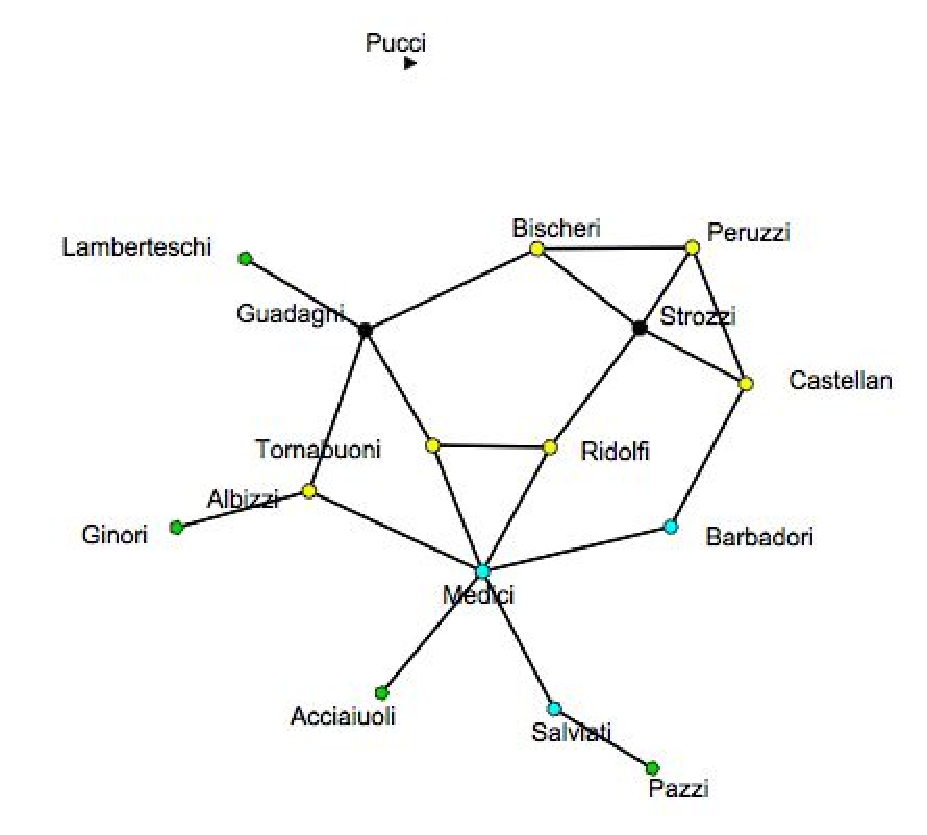
\includegraphics{myfigures/medici.eps}}
\end{center} 
\caption{Padgett's Renaissance Florentine family marriage network (1994).  Data set in \texttt{statnet} \citep{statnet:R}.} 
\label{fig1} 
\end{figure} 


  Although problems from sociology provide much of the motivations for social network analysis, network models can be applied to problems in a broad range of disciplines including political science, communications, marketing, and epidemiology.  Actors often represent individuals but they may also represent entities like nation-states, computers, or corporations.  The relation that connects actors is often friendship or actor $i$ ``liking" actor $j$ when the actors are individuals, but the tie can be any kind of relation such as a business transaction or the Internet connectedness between computers.  

Researchers have developed many \textit{descriptive} statistics that capture characteristics of an social network.  For example, the number of ties going to a particular actor is one measure of that actor's prestige in that network \citep{Wasserman:1994}.  Such statistics characterize properties of an observed network.  

In contrast, a statistical model can help us think about the distribution of possible unobserved outcomes.  It may illuminate local selection forces that shape the global structure of the network \citep{introp*, ergm}.  A good model will allow us to simulate a new network that retains some essential properties of the original network \citep{statnet}.  The challenge is to capture the interdependent nature of tie formation; in most social network environments, the chance that a tie will form between two actors $A$ and $B$ may be influenced by how likely a tie is to form between actors $B$ and $C$.  If we are looking at a monogamous marriage data set between individuals, the probability of Ross and Darrah being married will be highly affected by how likely Darrah and Nick are to be married!  Treating the ties as the response variable, the lack of independence between the ties marks a significant departure from the classical regression model where responses are treated as independent and raises the need for more complex models.  These complex models in turn require more sophisticated methods to calibrate them to the network data, a process that is still in its developmental stages as is evidenced by the stream of recent research on this topic \citep{Hunter:2006, Handcock:2006, recentp*, Morris:2008, Duijn:2009}.

In this proposal, we review the existing methods of finding parameter estimators for network models, including maximum pseudolikelihood estimators (MPLEs) and Markov chain Monte Carlo maximum likelihood estimators (MCMCMLEs).  We then present a simple algorithm that converges to the maximum likelihood estimators (MLEs) of a full exponential family distribution, the probability model underlying most social network models.  Unlike standard line search algorithms, our algorithm utilizes first derivative information only, evaluating neither the likelihood function itself nor derivatives of higher order than first which are expensive to compute when Markov chain Monte Carlo evaluation is used.


%%%%%%%%%%%%%%%%% SECTION %%%%%%%%%%%
\section{Introduction to Modeling}
Social networks are typically modeled as a random network represented by a matrix $Y$, an $n \times n$ matrix where $n$ is the number of actors.
Each entry $Y_{ij}$ in the random matrix $Y$ is a random variable representing a relation from actor $i$ to actor $j$, such that:
\[
	Y_{ij} = 
	\begin{cases}
		1 & \text{if a relationship exists \textit{from} actor $i$ \textit{to} actor $j$ (notation: $i \to j$)}\\
		0 & \text{otherwise}
	\end{cases}
	\
\]
where $i$ and $j$ take values in $1, \ldots, n$, $i \neq j$, for a network with $n$ actors.  Note that $Y_{ij}$ take only values of $0$ or $1$, reflecting our restriction on networks to those with dichotomous relations, that is, the relation between a pair of actors is either present or absent.  In addition, we do not allow the possibility of $i \to i$ and always denote $Y_{ii} = 0$.  In the special case that $Y_{ij} = Y_{ji}$ and thus the matrix $Y$ is symmetric, the network is referred to as a \textit{undirected} network or graph.  A network is \textit{directed} if it is not undirected.  

The exponential family random graph model (ERGM) commonly used in the network literature for $Y$ is as follows:
\begin{align}
	P_{\eta}(Y=y) &= \frac{ \exp(\eta^T g(y) ) }{ \kappa( \eta) } \qquad y \in \YY, \label{E:ERGM}
\end{align}
where $g(y)$ is a $q$-vector of statistics, $\eta$ is a $q$-vector of parameters, $\YY$ is the whole sample space of allowable networks which may contain $N = 2^{n(n-1)}$ networks if graphs are directed and $N = 2^{n(n-1)/2}$ if graphs are undirected, and $\kappa(\eta)$ is the normalizing constant such that
\begin{align*}
   \kappa(\eta) &= \int \exp [ \eta^T g(x) ] \, d \mu(x) %\label{E:kappa}
\end{align*}
where $\mu$ is a counting measure on $\YY$.  Thus an ERGM is a discrete exponential family distribution in canonical form \citep{tpe} and we will rely on many of the properties of exponential families.

We define the \textit{natural} parameter space $\Xi$ for $\eta$,
\begin{align}
   \Xi &= \{ \eta \in \RR^q : \kappa(\eta) < \infty \}.  \label{E:paramspace}
\end{align}
We find it also useful to define
\begin{align*}
	c(\eta) &= \log \kappa(\eta).
\end{align*}

Then our ERGM model \eqref{E:ERGM} can alternatively be expressed as 
\begin{align*}
	P_{\eta}(Y=y) &= \exp \left (\eta^T g(y) - c(\eta) \right ) \qquad y \in \YY.
\end{align*}
Also, we will frequently work with the log-likelihood of \eqref{E:ERGM}, that is,
\begin{align}
	\ell( \eta ) = \eta^T g(y) - c( \eta). \label{E:loglike}
\end{align}
%%%%%%%%% MAXIMUM ENTROPY APPROACH?
MAXIMUM ENTROPY?  \citep{Geyer:1992}[p. 666]

%%%%%%%%% NETWORK STATISTICS
A researcher specifies the statistics that compose the vector $g(y)$ in \eqref{E:ERGM} depending on what tie configurations he is concerned with modeling.  For example, a sociologist may be interested in the propensity for individuals to form reciprocal relations, where ties exist $i \to j$ and $j \to i$, or transitive relations, where ties exist $i \to j$, $j \to k$, $i \to k$.  The vector $g(y)$ can then be defined to be 
\begin{align*}
g(y) = \left ( \sum_{i<j} Y_{ij}Y_{ji}, \sum_{i \neq j \neq k} Y_{ij}Y_{jk}Y_{ik} \right )  
\end{align*}
where the components count the number of reciprocal and transitive tie configurations, respectively.  \citet{Wasserman:1996, Pattison:1999, logit, introp*} explore various network statistics that one might include in the vector $g(y)$.  

We will not discuss the merits or purpose of all the different network statistics here; what is important is that these statistics can be transparently calculated for a given network and the inclusion of them in $g(y)$, along with their parameters, allows the model to calculate probabilities of the presence of their associated tie formations.  In the works cited above, the researchers' primary consideration in defining a network statistic is to find a tie configuration that is of particular relevance to a problem.  For example, since reciprocity of ``liking" between individuals is commonly observed in friendship networks, it would be sensible to include a statistic for the number of reciprocal ties \citep{Holland:1981}.  Such a model, with parameters appropriately calibrated to a friendship network, might then generate networks that exhibit a significantly different number of reciprocal ties than would be expected in a uniformly random network.

%\begin{figure}[!h]
%\centering
%\scalebox{1}{\includegraphics{tableofstats.eps}}
%\caption{Table of some commonly used basic network statistics.}
%\label{fig2} 
%\end{figure}
%%%%%% TABLE OF COMMONLY USED NETWORK STATISTICS

  \citet{Handcock:2006, Hunter:2006, recentp*} continue the work of defining new network statistics but focus on the sensibility of the distributions generated from the specified models rather than just the scientific significance of certain tie configurations.  A complete description of network statistics is in \citet{Morris:2008}.  In addition, the issue of model selection between competing models has not been addressed though \citet{GOF} have begun making strides in this area.  Both of these areas are active area of research.

Finally, it should be noted that information about a particular node, say the gender for an individual, can be incorporated as \textit{covariate} data by allowing $g(y)$ to depend on a node-specific covariate matrix $X$.  Thus we may write $g(y, X)$ in place of $g(y)$ in \eqref{E:ERGM}.  We will continue to use $g(y)$ here for simplicity.


\section{Examples of ERGMs}

\subsection{Erd\H{o}s-R\'{e}nyi model}
The simplest example of an exponential random graph is the Erd\H{o}s-R\'{e}nyi model, also referred to as a Bernoulli network model, which assumes that all actors form a relation to other actors with the same probability, $p$ \citep{Wasserman:1994, ergm}.  The ERGM can be expressed as
\begin{align*}
	P_{\eta}(Y=y) &= \frac{ \exp(\eta g(y) ) }{ \kappa( \eta) } \qquad y \in \YY, 
\end{align*}
where the only statistic is a count of the number of edges for the network so that
\begin{align*}
%	g(y) = \frac{1}{N}\sum_{i \neq j} y_{ij},
	g(y) = \sum_{i \neq j} y_{ij}
\end{align*}
and the probability of a tie formation between any pair of actors is
\begin{align*}
	p = \frac{\exp(\eta)}{1+ \exp(\eta)}.
\end{align*}
As such, the $Y_{ij}$ are mutually independent of one another.  
The MLE of $\eta$ can found by taking the logit of the fraction of ties that are present in the data set, 
\begin{align*}
	\etaMLE = \logit \left ( \frac{\sum_{i \neq j} y_{ij}}{ N } \right )
\end{align*}
where $N = n(n-1)$, the number of possible ties in a network with $n$ actors.  The MLE for $\eta$ is easily calculated from the observed data but the independence assumption is too unrealistic for all but the simplest of cases; usually, a researcher is interested in the different probabilities of tie formations between actors.

\subsection{The $p_1$ Model}
\citet{Holland:1981} made advances in relaxing this independence assumption  with their $p_1$ model.  They focused on two empirical observations from sociometric studies:
\begin{itemize}
\item Reciprocation: there tend to be a ``surplus" of mutual relationships in network data sets compared to a uniform distribution of directed relationships.
\item Stars: some individuals attract a surplus of choices compared to a uniform distribution of directed relationships.
\end{itemize}
\citeauthor{Holland:1981} then constructed a family of distributions with parameters to control the probability of observing different numbers of mutual relationships and stars.  
Focusing on the \textit{dyad}, the set of a pair of actors and the possible relations between them, as the basic building block, they proposed the following model:
\[
	P( Y = y ) = \frac{1}{ K( \rho, \theta, \{ \alpha_i \}, \{\beta_j \} )}\exp \left \{  \rho m(y) + \theta y_{++} + \sum_i \alpha_i y_{i+} +  \sum_j \beta_j y_{+j}\right \}
\]
subject to $\sum_i \alpha_i = \sum_j \beta_j = 0$, where
\begin{align*}
	\rho &= \text{``force of reciprocation" or mutuality parameter}\\
	m(y) &= \sum_{i \neq j} y_{ij}y_{ji}, \quad \text{number of mutual relationships in $y$}\\
	\theta &= \text{``density" or overall choice effect parameter}\\
	y_{++} &= \sum_{i \neq j} y_{ij}, \quad  \text{total number of relations in $y$}\\
	\alpha_i &= \text{``productivity" or ``expansiveness" effect parameter for node $i$}\\
	y_{i+} &= \sum_{j} y_{ij}, \quad  \text{``out-degree" for node $i$ in $y$}\\
	\beta_j &= \text{``attractiveness" or ``popularity" effect parameter for node $j$} \\
	y_{+j} &= \sum_{i} y_{ij}, \quad  \text{``in-degree" for node $j$ in $y$}\\
	K &= \text{normalizing constant}
\end{align*}

By defining new dyad random variables, $D_{ij} = (Y_{ij}, Y_{ji} )$, \citeauthor{Holland:1981}  show that with some algebraic manipulation the form of the model above can be viewed as a log-linear model with independent dyad random variables, $D_{ij}$.  This makes it possible to use a logistic regression to calculate MLEs of the parameters.

The statistical independence at the dyad level, however, means that this model will not capture triangular tie configurations in which dyads are dependent.  Also, to reduce the number of parameters, the model assume $\rho_{ij} = \rho$, meaning that the tendency towards reciprocity is assumed to be the same across all actors.  Similarly, the model assumes that $\theta$ is the same across all actors.  This example illustrates how the parameter estimation methodology limits the scope of the model and what types of behavior it can capture.  

\subsection{Markov Graph Model}
\citet{Frank:1986} relax the independence assumption further with the implementation of \textit{Markov dependence} in which two dyads are independent, conditional on the rest of the graph, when they do not share a node.  The model use only three configurations in an \textit{undirected}, expressed as:
\[
	P( Y = y ) = \frac{1}{K( \theta, \sigma, \tau)}\exp \left \{ \theta L + \sigma S + \tau T	\right \} 
	\]
where
\begin{align*}
	\theta &= 		\text{Edge parameter} \\
	L &= 		\text{Number of edges} \\
	\sigma &= \text{2-Star parameter, propensity for individuals to have connections with two actors} \\
	S &= \text{Number of 2-stars ($i \leftrightarrow j$, $i \leftrightarrow k$) }\\
	\tau	&= \text{Triangle parameter, represents clustering} \\
	T &= \text{Number of triangles ($i \leftrightarrow j$, $j \leftrightarrow k$, $i \leftrightarrow k$)} \\
\end{align*}
None of the above parameters have subscript indices, reflecting the simplification from a \textit{homogeneity} assumption where parameters are equated if the configurations are the same ignoring the labels on the nodes (also called \textit{isomorphic} configurations.  In fact, this is the same simplification Holland and Leinhardt employ for the $\rho$ parameter in their $p1$ model.)  

The model is the first to break dyad independence, made possible by \citeauthor{Frank:1986}' methods of parameter estimation.  In particular, \citeauthor{Frank:1986} run Markov chain Monte Carlo simulations of the model at multiple values for a parameter to determine which fits the data best.  The authors also get maximum pseudolikelihood estimators (MPLE) obtained from a standard logistic regression and observe that the MPLEs are close to those from their simulations.  We will discuss the maximum pseudolikelihood methodology in the next section.  However, it may be noted here that it is this simplification of parameter estimation that has perpetuated the evolution of the network model to its general ERGM form \eqref{E:ERGM} that we consider in this paper.  
%More recent work has shown that this model with the exhibits problems with \textit{degeneracy} in which a model fit with parameters set to MLEs will generate only graphs that are empty or complete \citep{Handcock:Degeneracy}.  


%%%%%%%%%%%%%%%%% SECTION %%%%%%%%%%%

\section{Parameter Estimation}
Parameter estimation in statistical models is typically done through the method of maximum likelihood estimation in which values for the parameters, called maximum likelihood estimators (MLEs), that make the observed data most likely for the model are calculated.  Unfortunately, maximum likelihood for exponential families can be difficult for our model \eqref{E:ERGM} because the the normalizing constant $\kappa(\theta)$, a function of the very parameters we are trying to estimate, can be prohibitively expensive to evaluate.  For a directed network with $n$ actors, there are $N=2^{n(n-1)}$ different possible networks in our state space $\YY$, a huge number for even a moderate sized $n$.  It is for this reason that researchers like \citet{Holland:1981} made the restrictive assumptions of dyad independence for the $p_1$ model to enable the use of a logistic regression.  In this section we discuss the maximum pseudolikelihood and Markov chain Monte Carlo methods that have been developed to obtain estimators for the model parameters. 



\subsection{Maximum Pseudolikelihood method}
As mentioned in the previous section, \citet{Frank:1986} introduced the application of the maximum pseudolikelihood method, a method used in lattice systems \citep{Besag:1974}, to social network models.  \citet{Strauss:1990} further justify the use of maximum pseudolikelihood estimators (MPLE) as reasonable approximations for MLEs in social network models.  \citet{Wasserman:1996, Pattison:1999, logit} grasp the significance of this simplification and broaden the scope of network models to allow for any combination of network statistics, constrained only by the number of parameters. 

The method of maximum pseudolikelihood finds the values for the parameters that maximize the \textit{pseudolikelihood} or pseudo-loglikelihood functions for the given data set, which can be constructed from the distributions of a single tie, $Y_{ij}$, conditional on the rest of the network, which we will abbreviate as ``rest".  The conditional distribution of $Y_{ij} | \textrm{rest}$ is a Bernoulli distribution with log odds:
\begin{align}
	\log \left \{ \frac{P( Y_{ij} =1 | \textrm{rest} ) }{ P( Y_{ij} =0 | \textrm{rest} ) } \right \} = \eta^T \Delta(g(y))_{ij}, \label{E:logodds}
\end{align}
where we define the vector of \textit{change statistics}, $\Delta(g(y))_{ij}$, to be
%which is the change in $g(y)$ when $y_{ij}$ changes from 0 to 1 while the rest of the network remains the same,  
\begin{align*}
	\Delta(g(y))_{ij} = g(y_{ij}^+) - g(y_{ij}^-)
\end{align*}
where $y_{ij}^+$ and $y_{ij}^-$ represent networks with $y_{ij} = 1$ or $y_{ij} = 0$, respectively, while leaving the rest of the network as $y$.  Thus $\Delta(g(y))_{ij}$ is the change in $g(y)$ when $y_{ij}$ changes from 0 to 1.

The pseudolikelihood is constructed from \eqref{E:logodds} by assuming that the $Y_{ij}$ are in fact mutually independent, that is, 
\begin{align*}
	P( Y_{ij} =1 | \textrm{rest} ) = P( Y_{ij} =1 ).
\end{align*}
With this independence assumption, \eqref{E:logodds} is exactly the setup for a logistic regression through which we can get the estimates of $\eta$, called the maximum pseudolikelihood estimators, or MPLEs.  In the case where the dyads are in fact independent, the MPLEs will equal the MLEs.  \citet{Strauss:1990} show that in many cases with dyad dependence, MPLE still yield reasonable approximations of the true MLEs for social network models.  However, \citet{Geyer:1992, Snijders:2002, Duijn:2009} demonstrate that MPLEs can produce very misleading results, and social network software packages such as \texttt{statnet} in the \texttt{R} platform now use MLE methods rather than MPLE \citep{statnet:R}.  

\subsection{Markov chain Monte Carlo methods}
\citet{Geyer:1992, Corander:1998, Snijders:2002} developed Markov chain Monte Carlo (MCMC) methods to approximate the MLE of an exponential family.  Of these, \citeauthor{Geyer:1992}'s MCMCMLE method appears to be most commonly implemented in the literature and software \citep{Hunter:2006, Handcock:2006, ergm, statnet, GOF}.  

Rather than maximizing the log-likelihood \eqref{E:loglike},
\[	\ell(\eta ) = \eta ^T g(y) - c(\eta) \]
with respect to $\eta$, \citeauthor{Geyer:1992} fix $\eta^0$ at a known value and look to maximize the log of the likelihood ratio\footnote{In fact, $r(\eta, \eta^0)$ is also a log-likelihood.  The addition to $\ell (\eta)$ of an arbitrary function of data that does not contain the parameter $\eta$ will still observe the definition of a log-likelihood.}, $r( \eta, \eta^0 )$.
\begin{align}
 r( \eta, \eta^0 ) &= \ell( \eta ) - \ell( \eta^0 ) \notag \\ 
					&= ( \eta - \eta^0)^T g(y) - \log \left [ \exp \{ c(\eta) - c(\eta^0) \} \right ]. \label{E:r}
\end{align}
The approach then focuses on approximating the ratio of normalizing constants, $\frac{ \exp \{c(\eta) \} }{ \exp \{c(\eta^0) \} }$.  The value of $\eta$ that maximizes the approximation of $r( \eta, \eta^0 )$ is then a good estimate of the MLE when it exists.  This can be seen by starting with the normalizing constant,
\begin{align*}
	\exp \{c(\eta) \} &= \int \exp\{\eta^Tg(x)\} \, d\mu(x).
\end{align*}
The ratio of normalizing constants is then
\begin{align*}
	\exp\{ c(\eta) - c(\eta^0) \} &= \frac{ \int \exp\{\eta^Tg(x)\} \, d\mu(x) }{ \exp\{ c(\eta^0) \} } \\
	&= \frac{ \int \exp\{( \eta - \eta^0)^T g(x) + (\eta^0)^Tg(x)\}\, d\mu(x)  }{ \exp\{ c(\eta^0) \} } \\
	&= \int \exp\{( \eta - \eta^0)^T g(x) \} \frac{ \exp \{(\eta^0)^T g(x)\} }{ \exp\{ c(\eta^0) \}  } \, d\mu(x)\\
	&= \E_{\eta^0} \left [ \exp\{ ( \eta - \eta^0)^T g(Y)  \} \right ].
\end{align*}

By the Markov chain strong law of large numbers (or Birkhoff ergodic theorem), this expectation can be approximated by the sample mean for large sample size,
\begin{align*}
	&\approx \frac{1}{m} \sum_{i=1}^{m}\exp \{ ( \eta - \eta^0)^Tg(Y_i) \}
\end{align*}
where $Y_1, \ldots, Y_m$ are draws from the exponential family distribution with parameter $\eta^0$.  This sample can be generated using Markov chain Monte Carlo method such as a Metropolis algorithm.

Thus, $r( \eta, \eta^0 )$ can be approximated by
\begin{align}
\hat{r}_m( \eta, \eta^0 ) &= ( \eta - \eta^0)^Tg(y) - \log \left [ \frac{1}{m} \sum_{i=1}^{m} \exp \{ ( \eta - \eta^0)^Tg(Y_i)\} \right ] \label{E:r_hat}
\end{align}
and 
\begin{align*}
	\hat{r}_m( \eta, \eta^0 ) \to r( \eta, \eta^0 ) \text{ a.s. as $m \to \infty$}.
\end{align*}

If we call the maximizer of \eqref{E:r_hat} $\hat{\eta}_m$ and assume that the MLE $\etaMLE$ exists, \citeauthor{Geyer:1992} show that 
\begin{align*}
\hat{\eta}_m \to \etaMLE \quad a.s.
\end{align*}
 whenever the Markov chain is ergodic. 

In practice, \citeauthor{Geyer:1992} recognize that ``enormous" Monte Carlo sample sizes may be necessary and that best results are obtained when $\eta^0$ is near $\etaMLE$---a condition that of course cannot be checked since $\etaMLE$ is unknown!  In addition, \citeauthor{Geyer:1992} recommend iterating the algorithm several times, where each successive value will be closer to $\etaMLE$ than the previous.  At the time of this writing, the MCMCMLE routine in \texttt{statnet} uses by default 10,000 Monte Carlo samples and a maximum of three iterations \citep{statnet:R}, using the MPLE as the initial value for $\eta^0$.  We follow up with an example presented by \citet{ergm} in \texttt{statnet} in which the MCMCMLE procedure can fail.

\vspace*{0.2in}

\textbf{Sampson's Monastery Data set}

\begin{figure} 
\begin{center} 
\scalebox{.6}{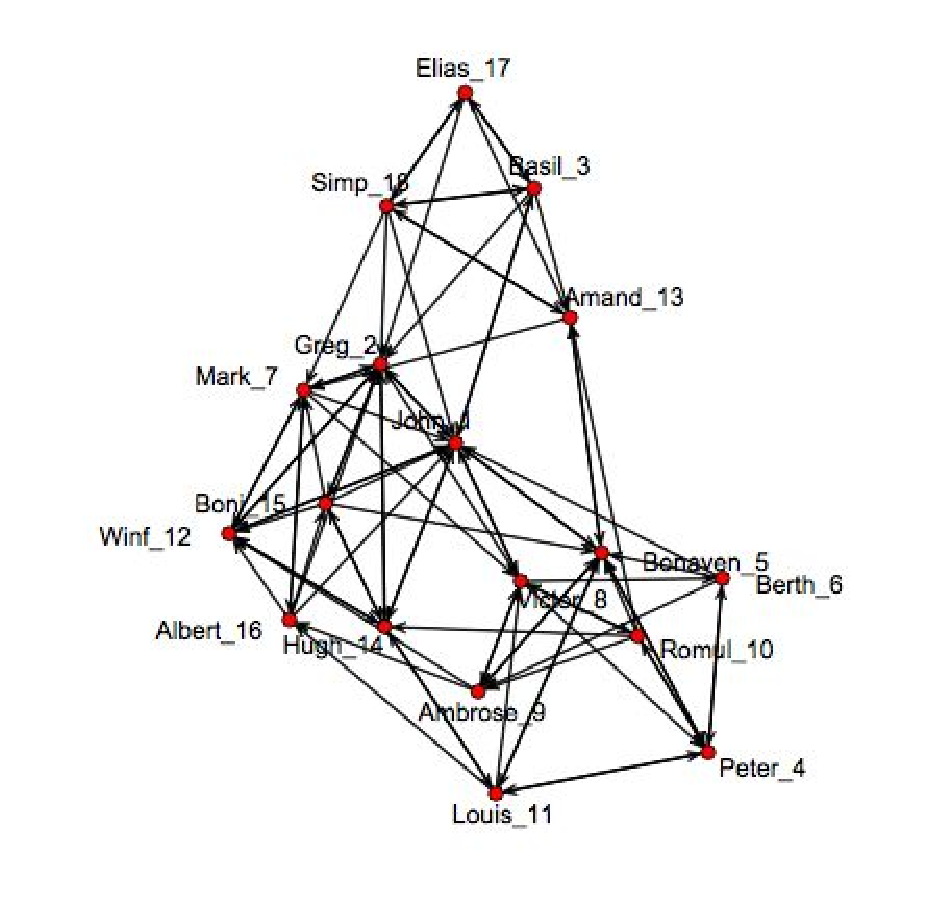
\includegraphics{myfigures/samplike.eps}}
\end{center} 
\caption{Sampson's monastery affinity network (1969).} 
\label{fig-samplike} 
\end{figure} 

\citeauthor{ergm} illustrate the practical difficulty associated with a poor initial value in the MCMCMLE algorithm with Sampson's monastery data set, a standard data set in the social network literature which we depict in Figure \ref{fig-samplike}.  The network is directed with 18 actors and 88 ties present out of $18(17)=306$ possible ties.  For this data set \citeauthor{ergm} use the simple Erd\H{o}s-R\'{e}nyi model described earlier, with the network statistic $g(y)$ equal to the total number of edges present, so $g(y_{obs}) = 88$.  The true MLE is equal to $\logit(88/306) = -0.9072$.  When $\eta^0$ is chosen to be $1$, however, \citeauthor{ergm} demonstrate that the algorithm will fail in a single iteration.  With $\eta=1$, the model describes that each of the 306 possible edges will occur independently with probability $p = \frac{1}{1+e^{-\eta}} = \frac{1}{1+e^{-1}} = 0.731$.  The problem arises from the fact that this is a high probability relative to the observed data set, which suggests a much smaller probability of tie formation of $88/306= 0.288$.  In fact, the probability of obtaining $g(Y) < g(y_{obs})=88$ is close to zero at $2.3 \times 10^{-59}$, where $g(Y)$ are generated from a binomial distribution with $n=306$, $p =0.731$.  The MCMCMLE algorithm looks to maximize the approximated log likelihood ratio \eqref{E:r_hat}, but if the MC sample is unable to generate $g(Y)< g(y_{obs})$, \eqref{E:r_hat} will not have a maximizer since the function will not have a point where the derivative is zero (see upper solid line in Figure \ref{F:bad eta}).  The problem is not present when an initial value close to the true MLE like $\eta^0 = -1$ is used (lower solid line in Figure \ref{F:bad eta}).  With the default three iterations in the \texttt{statnet} software, the algorithm gets to $\eta = -0.364$, but with 10 iterations it arrives at the MLE.

\begin{figure} 
\begin{center} 
\scalebox{.8}{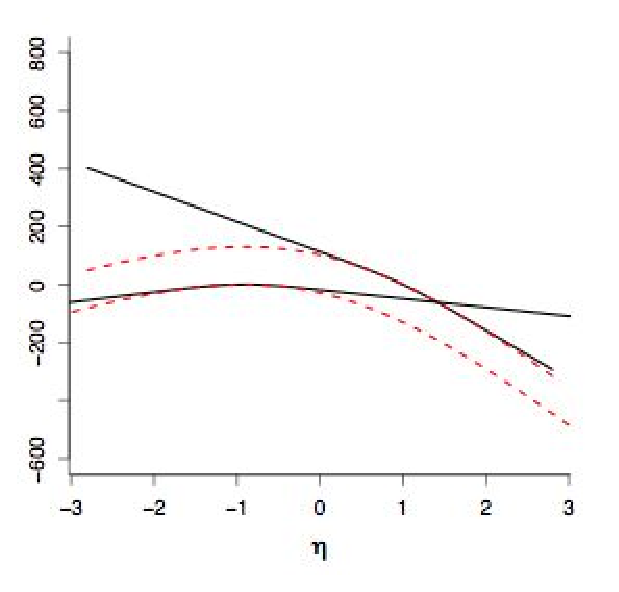
\includegraphics{myfigures/bad_eta.eps}}
\end{center} 
\caption{Log likelihood ratios for different values of $\eta$ for the Sampson Monastery data set.  Dotted lines are exact log likelihood ratios, solid lines are the approximation by \eqref{E:r_hat}.  Upper solid and dotted lines correspond to $\eta^0 = 1$, lower lines correspond to $\eta^0 = -1$.  The upper solid line, the approximate log likelihood ratio with $\eta^0 = 1$, has no maximizing value of $\eta$ \citep{ergm}.} 
\end{figure} 

%\begin{align*}
%\hat{r}_m( \eta, \eta^0 ) &= ( \eta - \eta^0)^Tg(y) - \log \left [ \frac{1}{m} \sum_{i=1}^{m} \exp \{ ( \eta - \eta^0)^Tg(Y_i)\} \right ] 
%\end{align*}

% DEFINITIONS OF CONCEPTS
\section{Definitions and Theorems}

We will need to state some definitions and theorems to further discuss the conditions for finding MLEs for ERGMs.

%convex set - 
\begin{definition}
A set $C \subset \RR^n$ is \textbf{convex} if it includes for every pair of points the line segment that joins them.  In other words, if for every choice of $x_0, x_1 \in C$, one has $[x_0, x_1] \subset C$, or
\begin{align*}
	(1 - \tau) x_0 + \tau x_1 \in C \quad \text{for all $\tau \in (0,1)$}
\end{align*}
\citep{Rockafellar}.
\end{definition}

%convex function - 
\begin{definition}
An extended real-valued function $f$ on a convex set $C$ is a \textbf{convex function} relative to $C$ if for every choice of $x_0, x_1 \in C$, one has 
\begin{align*}
	f( (1-\lambda) x_0 + \lambda x_1) \leq (1- \lambda) f(x_0) + \lambda f(x_1) \quad \text{for all $\lambda \in (0,1)$}
\end{align*}
and $f$ is strictly convex relative to $C$ if this inequality is strict for points $x_0 \neq x_1$
\citep{Rockafellar}.
\end{definition}

\begin{definition}
The \textbf{epigraph} of $f$ is the set
\begin{align*}
	\textrm{epi} f = \{(x, \alpha ) \in \RR^n \times \RR | \alpha \geq f(x) \}
\end{align*}
The epigraphs consist of all the points of $\RR^{n+1}$ lying on or above the graph of $f$
\citep{Rockafellar}.
\end{definition}

% dom f
\begin{definition}
The \textbf{effective domain} of a function $f:\RR^n \to \bar{\RR}$ is the set
\begin{align*}
	\dom f = \{ x \in \RR^n | f(x) < \infty \}
\end{align*}
\citep{Rockafellar}.
\end{definition}


% proper
\begin{definition}
A convex function $f$ is said to be \textbf{proper} if its epigraph is non-empty and contains no vertical lines, i.e. $f(x) < \infty$ for at least one $x$ and $f(x) > - \infty$ for every $x$
\citep{Rockafellar:1970}.
\end{definition}

%convex hull - 
\begin{definition}
The \textbf{convex hull} of a set $C \subset \RR^n$, denoted by \conhull C$, is the smallest convex set that includes $C$
\citep{Rockafellar}.
\end{definition}


%convex support -
\begin{definition}
Let $Y$ be distributed as an ERGM as defined in \eqref{E:ERGM}.  If $C$ is the smallest closed convex set such that the natural statistic $g(Y) \in C$ with probability one under some distribution in the family, in which case this holds for all distributions in the family, then $C$ is called the \textbf{convex support} of the family \citep{Barndorff, Geyer:1990}.  Here,
\begin{align*}
	C = \conhull g(S)
\end{align*}
where $g(S) = \{ g(s) \: s \in S \}$ and $S = 2^E$, where $E$ are edge indices in the graph and $2 = \{0,1\}$.
\end{definition}


%cone - A cone is a set $\FF$ with the property that for all $x \in \FF$,
%\begin{align*}
%	x \in \FF \Rightarrow \alpha x \in \FF, \quad \text{for all $\alpha \geq 0$.}
%\end{align*}

%tangent cone - The tangent cone of a set $C \subset \RR^n$ at a point $x \in C$, denoted $T_C(x)$, is the set of all vectors $v$ such that there exists a sequence $\tau_n \downarrow 0$ and a sequence $x_n$ in $C$ converging to $x$ such that 
%\begin{align*}
%	\frac{x_n - x}{\tau_n} \to v
%\end{align*}
%\citep{Geyer:2001}

%normal cone - The \textit{regular normal cone} of a set $C \subset \RR^n$ at a point $x \in C$, denoted $\hat{N}_C(x)$, is the set of all vectors $v$ such that  
%\begin{align*}
%	\langle v, y -x \rangle \leq o( |y -x | ), 	\quad y \in C.
%\end{align*}
%The \textit{normal cone} of a set $C \subset \RR^n$ at a point $x \in C$, denoted $N_C(x)$, is the set of all vectors $v$ such that there exists a sequence $x_n$ in $C$ converging to $x$ and a sequence $v_n \to v$ with $v_n \in \hat{N}_C(x_n)$.
%\citep{Geyer:2001}

%polar - 


%level set 
\begin{definition}
A \textbf{level set} of a function $f$ is the set of $x$ such that
\begin{align*} 
	\lev_{\leq \alpha} f = \{ x \in \RR^n | f(x) \leq \alpha \}
\end{align*}
\citep{Rockafellar}.  For convex functions we will typically be interested in $\lev_{\leq \alpha} f$, for concave functions we will typically be interested in $\lev_{\geq \alpha} f$, defined similarly.
\end{definition}

%\begin{definition}
%A function $f:\RR^n \to \bar{\RR}$ is \textbf{(lower) level-bounded} if for every $\alpha \in \RR$, the set $\lev_{\leq \alpha} f$ is bounded (possibly empty)
%\citep{Rockafellar}[p. 11].
%\end{definition}


%lower limit \citet[p8]{Rockafellar}
%lower limit of $f$
%\begin{align*}
%	\liminf_{x\to \bar{x}} f(x) = \lim_{\delta \searrow 0} \left [ \inf_{ x\in B(\bar{x}, \delta )} f(x) \right ]
%\end{align*}

%lower semincontinuous 
\begin{definition}
The function $f$ is \textbf{lower semicontinuous (lsc)} at $\bar{x}$ if
\begin{align*}
	\liminf_{x\to \bar{x}} f(x) \geq f(\bar{x})
\end{align*}
\citep[p8]{Rockafellar}.  If a function $f$ is continuous at $\bar{x}$, it is lsc at $\bar{x}$.
\end{definition}

%affine set - 

%affine hull - 
\begin{definition}
The \textbf{affine hull} of a convex set $C$ is the smallest affine set that includes $C$.  It is the set of all affine combinations of elements of $C$, that is,
\begin{align*}
	\aff(C) = \left \{ \sum_{i=1}^{k} \alpha_i x_i | x_i \in C, \, \alpha_i \in \RR, \, \sum_{i=1}^{k} \alpha_i = 1, \, k = 1, 2, \ldots \right \}
\end{align*}
\citep{Rockafellar}.
\end{definition}

\begin{definition}
For a set $C \subset \RR^n$, the interior of $C$ is defined to be
\begin{align*}
%	\cl \, C &= \text{closure of $C$}  = \{ x | \, \forall V \in \NN(x), \, V \cap C \neq \emptyset \}
	\intr \, C &= \{ x | \, \exists V \in \NN(x), \, V \subset C \} 
%	\bd \, C &= \text{boundary of $C$}  = \cl C  \backslash \intr C
\end{align*}
	where $V \in \NN(x) =$ the collection of all neighborhoods of $x$.  The \textbf{relative interior} of $C$, $\rintr \, C$, is the interior of $C$ relative to its affine hull
\citep{Rockafellar}.
\end{definition}

%direction of constancy
%direction of recession
\begin{definition}
A vector $\delta$ is a \textbf{direction of recession} of a concave function $\ell$ if for every $\eta \in \Xi$, the function $\ell(\eta + s \delta)$ is a nondecreasing function of $s$.

A vector $\delta$ is a \textbf{direction of constancy} of a convex or concave function $\ell$ if for every $\eta \in \Xi$, the function $\ell(\eta + s \delta)$ is a constant function of $s$.  

Note that every direction of constancy is a direction of recession
\citep{Geyer:2009}.
\end{definition}

%minimal - 
\begin{definition}
An exponential family is said to be \textbf{minimal} if the log likelihood has no direction of constancy  
\citep{Geyer:2009}.  Alternatively, the representation of an ERGM random variable $Y$ defined by \eqref{E:ERGM} is said to be minimal if neither the natural statistics $g(y)$s nor the $\eta$s satisfy a linear constraint \citep{tpe}.
\end{definition}

% full, regular
\begin{definition}
An exponential family is \textbf{full} if its natural parameter space is as large as possible, as defined in \eqref{E:paramspace} 
\begin{align*}
   \Xi &= \{ \eta \in \RR^q : \kappa(\eta) < \infty \}.  
\end{align*}
If, in addition, the natural parameter space $\Xi$ is a $q$-dimensional \textit{open} set, the exponential family is said to be \textbf{regular}.  The natural parameter space for an ERGM is $\RR^q$ since $\kappa(\eta)$ is a finite sum of finite values.  Thus ERGMs are regular.
\end{definition}

%steep

%Lipschitz
\begin{definition}
A function $f$ is \textbf{Lipschitz continuously differentiable} on an open set $N$ if there exists a constant $L > 0$ such that
	\begin{align*}
		|| \nabla f(x) - \nabla f(\tilde{x}) || \leq L || x - \tilde{x} || \quad \text{for all $x, \tilde{x} \in N$}
	\end{align*}
	\citep{NW}.
\end{definition}



%%%%%%%%%%%%%%%%% SECTION %%%%%%%%%%%

%\section{Theorems for Line Search Algorithm}

%\begin{theorem}[Theorem 10.4, p. 86 from \citet{Rockafellar:1970}] \label{Thm:Lipschitzian}
%Let $f$ be a proper convex function, and let $S$ be any closed bounded subset of $\dom \, f$.  Then $f$ is Lipschitzian relative to $S$.
%\end{theorem}

\begin{theorem}[Theorem 1.6 from \citet{Rockafellar}] \label{Thm:lsc epi}
 The following properties of a function $f: \RR^n \to \bar{\RR}$ are equivalent:
 \begin{enumerate}
	\item $f$ is lower semicontinuous on $\RR^n$
	\item the epigraph set $\epi f$ is closed in $\RR^n \times \RR$
	\item the level sets of type $\lev_{\leq \alpha} f$ are all closed in $\RR^n$
 \end{enumerate}
%This means that the function is continuous with the exception of jump discontinuities (left and right limits exist, but are not equal) where the open point is on the upper piece and the solid point is on the lower piece.
\end{theorem}

%\begin{theorem}[Theorem 1.9 from \citet{Rockafellar}] \label{Thm:compact}
%	Suppose $f:\RR^n \to \bar{\RR}$ is lower semi-continuous, level-bounded and proper.  Then the value $\inf f$ is finite and the set argmin $f$ is nonempty and compact.
%\end{theorem}

\begin{prop}[Proposition 2.7 in \citet{Rockafellar}] \label{Prop:convex lev}
For a concave function $f: \RR^n \to \bar{\RR}$ all level sets of type $\lev_{\geq \alpha} f$ and $\lev_{> \alpha} f$ are convex.
\end{prop}

\begin{corollary}[Corollary 8.7.1 in \citet{Rockafellar:1970}, p. 70] \label{Cor:bounded lev}
Let $f$ be a closed proper convex function.  If the level set $\lev_{\leq \alpha} f$ is non-empty and bounded for one $\alpha$, it is bounded for every $\alpha$.
\end{corollary}

\begin{lemma}[ Lemma 2.7.1 from \citet{tsh}]
The natural parameter space of an exponential family is convex.
\end{lemma}

\begin{theorem}[ Theorem 4.1 from \citet{tpe}] \label{Thm:infinitely-differentiable}
For any integrable function $f$ and any $\eta$ in the interior of $\Xi$, the natural parameter space of $\eta$, the integral,
\begin{align}
	\int f(x) \exp [ \eta^Tg(x) ] d\mu(x)
\end{align}
is continuous and has derivatives of all orders with respect to the $\eta$'s, and these can be obtained by differentiating under the integral sign.	Here $\mu$ is a measure such that $\int \exp [ \eta^Tg(x) - c(\eta)] d\mu(x) = 1$.
\end{theorem}

\begin{corollary} \label{Cor:infinitely-differentiable}
Then (assuming $\Xi$ is nonempty) define
$$
   p_\eta(x) = \frac{1}{\kappa(\eta)} \exp [ \eta^T g(x) ]
$$
For each $\eta \in \Xi$, the function $p_\eta$ is a probability density
function with respect to $\mu$, and for any function real-valued function $f$,
$$
   E_\eta\{ f(X) \} = \int f(x) \exp [ \eta^T g(x) - c(\eta) ] \, d \mu(x)
$$
(assuming the expectation exists).  Then for
any $\eta_0$ in the interior of $\Xi$ and
for any function $f$ such that $E_{\eta_0}\{ f(X) \}$ is finite, the
function $\eta \mapsto E_\eta\{ f(X) \}$ is infinitely differentiable at
$\eta_0$ and derivatives can be obtained by differentiating under the integral
sign.  
\end{corollary}

\begin{corollary} \label{Cor:Lipschitzian}
Let the function $p_\eta$ and $\Xi$ be defined as above.  Then for
any $\eta_0$ in the interior of $\Xi$ and
for any function $f$ such that $E_{\eta_0}\{ f(X) \}$ is finite, the derivatives of the function $\eta \mapsto E_\eta\{ f(X) \}$ are Lipschitzian relative to any \emph{compact} subset of the interior of $\Xi$.
\end{corollary}
This follows by the continuity of the derivative and the subsequent application of the mean value theorem over a compact set which guarantees the maximum and minimum values are attained.

\begin{corollary} \label{Cor:ExpFam_Deriv}
For 
the ERGM described by \eqref{E:ERGM},
\begin{align}
	\E_\eta(g_j(Y)) &= \pderiv{c(\eta)}{\eta_j}  \label{E:Expectation}\\
%	\intertext{and}
	\Cov_\eta  ( g_j(Y), g_k(Y)  ) &= \ppmderiv{ c(\eta) }{\eta_j}{\eta_k} \label{E:Cov}
\end{align}

Then defining the gradient operator $\nabla = \left [ \pderiv{}{\eta_j} \right ]$,
\begin{align*}
	\E_\eta(g(Y)) &= \nabla c(\eta)	\\
	\Var_\eta(g(Y)) &= \nabla^2 c( \eta ). 	\label{E:Varmat}
\end{align*}
\end{corollary}

%\begin{proof}
%Beginning with
%\begin{align*}
%&\int \exp [ \eta^Tg(x) - c(\eta)] d\mu(x) = 1,
%\intertext{we take partial derivatives of each side so that}
%\pderiv{}{\eta_j} &\int \exp [ \eta^Tg(x) - c(\eta)] d\mu(x) = 0
%\end{align*}

%By the previous corollary, we can differentiate under the integral sign so that,
%\begin{align*}
%&\int \pderiv{}{\eta_j}\exp [ \eta^Tg(x)] \exp [- c(\eta)] d\mu(x) = 0 \\
%&\int g_j(x) \exp [ \eta^Tg(x)]\exp [- c(\eta)]  - \pderiv{}{\eta_j} c( \eta) \exp [ \eta^Tg(x)] \exp [- c(\eta)] d\mu(x) = 0 \\
%&E_\eta g_j(X)  - \pderiv{}{\eta_j} c( \eta) \cdot 1 = 0 \\
%&E_\eta g_j(X) = \pderiv{c(\eta)}{\eta_j} 
%\end{align*}
%which is the first result.  To get the second result, we take the partial derivative of this first result with respect to $\eta_k$, so that
%\begin{align*}
%	\ppmderiv{c(\eta)}{\eta_j}{\eta_k}  &= \pderiv{}{\eta_k}\int g_j(x) \exp [ \eta^Tg(x)]\exp [- c(\eta)] d\mu(x) \\
%	&= \int g(x)_j \pderiv{}{\eta_k} \exp [ \eta^Tg(x)]\exp [- c(\eta)] d\mu(x) \\
%	&= \int g(x)_j \bigg ( g(x)_k \exp [ \eta^T g(x)]\exp [- c(\eta)] \notag \\ &-  \pderiv{c( \eta)}{\eta_k}  \exp [ \eta^Tg(x)] \exp [- c(\eta)] \bigg ) d\mu(x) \\
%	&= E_\eta(g_j(X) g_k(X))-  E_\eta(g_k(X)) \cdot E_\eta(g_j(X)) \\
%	&= \Cov_\eta( g_j(X), g_k(X) )
%\end{align*}
%as desired.
%\end{proof}

\begin{theorem} \label{Thm:loglike concave}
The log-likelihood function
\begin{align*}
	\ell( \eta ) = \eta^T g(y) - c( \eta)
\end{align*}
for a full exponential family is concave with respect to the parameter $\eta$.  The log-likelihood is strictly concave if and only if the family is minimal \citep{Geyer:gdor}.
\end{theorem}

%\begin{trivlist}
%\item \textbf{Comment by Charlie:}
%This theorem, as stated, is false.  Fortunately, your proof doesn't prove this.
%So you proof is not incorrect.  See my thesis for the correct version.
%By the condition for equality in H\"{o}lder's inequality, the log likelihood
%fails to be strictly convex if and only if $(\eta_1 - \eta_2)^T g(X)$ is
%almost surely constant with respect to any distribution in the exponential
%family.  If is an additional condition (usually called ``minimality'' of
%the exponential family) that one does not have $\zeta^T g(X)$ almost surely
%constant for any nonzero vector $\zeta$ or equivalently that $\nabla^2 c(\eta)$
%is a strictly positive definite matrix for any $\eta$ in the interior of
%$\Xi$ (assuming that the interior is nonempty).
%\end{trivlist}

%\begin{proof}
%(Partial) The first term in the log-likelihood, $\eta^T g(y)$, is linear and thus concave and convex.  It remains to show then that the second term, $-c( \eta)$, is concave, or that $c( \eta)$ is convex.  That is, we wish to show that
%\begin{align*}
%	c( \alpha \eta_1 + (1-\alpha) \eta_2 ) &\leq \alpha c( \eta_1) + (1-\alpha)c(\eta_2) \qquad \text{for $0 \leq \alpha \leq 1$},\\
%	\intertext{or that}
%	\exp \{ c(\alpha \eta_1 + (1-\alpha) \eta_2) \} &\leq \exp \{ \alpha c( \eta_1) \} \exp \{ (1-\alpha)c(\eta_2) \}.
%\end{align*}

%Working with the left-hand side of the expression above,
%\begin{align*}
%	\exp \{ c(\alpha \eta_1 + (1-\alpha) \eta_2) \} &= \kappa( \alpha \eta_1 + ( 1- \alpha) \eta_2 ) \\
%	&= \int \exp \{ \alpha \eta_1 + (1-\alpha) \eta_2)^T g(x) \} d\mu(x) \\
%	&= \int \exp \{ \alpha \eta_1^T g(w) \} \exp \{(1-\alpha)\eta_2^T g(x) \} d\mu(x)	\\
%	&= \int \left (e^{ \eta_1^T g(w)} \right )^\alpha  \left ( e ^{ \eta_2^T g(w) } \right )^{1-\alpha} d\mu(x) \\
%	\intertext{H\"{o}lder's inequality states that for $p$, $q > 0$,}
%	\int a_k b_k d\mu(x) &\leq \left ( \int a_k^p d\mu(x) \right )^{\frac{1}{p}} \left ( \int b_k^q d\mu(x) \right )^{\frac{1}{q}}.
%	\intertext{Letting $p = 1/\alpha$ and $q = 1 / (1- \alpha)$ and applying this inequality, our last expression becomes}
%	&\leq \left( \int e^{ \eta_1^T g(w)} d\mu(x) \right )^\alpha  \left ( \int e ^{ \eta_2^T g(w) } d\mu(x) \right )^{1-\alpha} \\
%	&= \kappa( \eta_1 )^\alpha \kappa( \eta_2) ^{1 - \alpha} \\
%	&= \exp \left ( \log \left \{ \kappa( \eta_1 )^\alpha \kappa( \eta_2) ^{1 - \alpha} \right \} \right )\\
%	&= \exp \left ( \alpha \log \kappa( \eta_1 ) + (1 - \alpha) \log \kappa( \eta_2) \right )\\
%	&= \exp \{ \alpha c( \eta_1 ) \} \exp \{ (1 - \alpha) c( \eta_2) \}.
%\end{align*}
%as desired.
%\end{proof}

\begin{theorem}[Existence and Uniqueness of MLE]
For a regular exponential family, if $y$ is the observed data, $g(y)$ the natural statistic, $C$ the convex support, then the MLE exists and is unique if and only
if $g(y) \in \rintr \, C$ \citep{Barndorff}[Corollary 9.6].
\end{theorem}
Equivalently, \citet{Geyer:gdor} approaches the existence and uniqueness of the MLE from the perspective of directions of constancy and recession of the log-likelihood, as follows:

\begin{theorem}[Theorem 4, \citep{Geyer:gdor}]
For a full exponential family with convex support $C$ and observed value of the natural statistic $g(y)$ such that $g(y) \in C$, the MLE exists if and only if every direction of recession is a direction of constancy.  
\end{theorem}

When the MLE does not exist for an exponential family, and thus there exists a direction of recession that is not a direction of constancy, \citet{Geyer:2009} shows that the MLE exists in the \textit{limiting condition model}, which is itself an exponential family in which the MLE will always exist.  

\begin{theorem}[MLE Expectation Equation] \label{Thm:MLE of ERGM}
For the ERGM described by \eqref{E:ERGM}, the MLE for $\eta$, $\etaMLE$, will be attained when
\begin{align}
	E_{\etaMLE} g_j(Y) = g_j(y)
\end{align}
provided the MLE exists.  This result is sometimes referred to as the Expectation equation.
\end{theorem}

%\begin{proof}
%We take the log-likelihood \eqref{E:loglike},
%\begin{align*}
%	\ell( \eta ) &= \eta^T g(y) - \log \kappa( \eta)
%	\intertext{set the first partial derivative equal to zero and solve for $\eta$ that fulfills this condition.  By the previous theorem, since we know that \eqref{E:loglike} is strictly concave, we know that we will have found the maximum.}
%	\pderiv{\ell}{\eta_j} &= g_j(y) - \pderiv{c(\eta)}{\eta_j} \stackrel{set}{=} 0 \\
%	\pderiv{}{\eta_j}c(\eta) &= g_j(y) \\
%	E_{\etaMLE} g_j(Y) &= g_j(y)
%\end{align*}
%as desired.
%\end{proof}


%%%%%%%%%%%%% CH 2.  ALGORITHM CONVERGENCE %%%%%%%%%%%%%%%%%%%%%%%%%
\setstretch{1}
\chapter{New Algorithm and its Convergence}
\setstretch{1.5}
\section{Algorithm Outline}
We propose a simple algorithm based on Theorem \ref{Thm:MLE of ERGM} that converges to the MLE of a regular exponential family when the MLE exists and is unique.  It avoids evaluation of the the likelihood and uses the gradient to direct the search as well as indicate how far the current estimate is from the true MLE.  The algorithm is a line search with updates of the form
\begin{align*}
	\eta_{k+1} &= \eta_k + \alpha_k p_k
\end{align*}
where $\alpha_k$ is the \emph{step length}, and $p_k$ is the \emph{search direction}.
 
We use the notation established earlier, $\ell(\eta)$ for the log-likelihood, and $\nabla \ell( \eta)$ for the gradient of the log-likelihood. The algorithm is as follows:

% ALGORITHM 

Get an initial value, $\eta_0$.\\ 
Set $k=0$. \\
Set $p_k = \nabla \ell( \eta_k)$, the direction of steepest ascent. \\
\textbf{while}  $\parallel \nabla \ell( \eta_k) \parallel > \epsilon$ \\ 
\hspace{4mm} \indent	 \textbf{Find} the step size $\alpha_k$ that satisfies the \textit{curvature condition}
\begin{align*}
	 0 & \leq \nabla \ell( \eta_k + \alpha_k p_k)^T p_k \leq c \nabla \ell(\eta_k)^T p_k
\end{align*}
\indent for some $0 < c < 1$.  This condition requires $\alpha_k$ to fall within the acceptable region in Figure \ref{F:alpha_region}. \\

\begin{figure}[!h]
\centering
    \scalebox{.4}{\input{myfigures/alphamax.pstex_t}}
	\caption{The curvature condition for $\alpha$.}
\label{F:alpha_region}
\end{figure}

$\eta_{k+1} = \eta_k + \alpha_k p_k$.\\
\indent $\nabla \ell( \eta_{k+1}) = g( y _{obs}) - \E_{\eta_{k+1}}g(Y)$.\\
\indent \textbf{Find} the new search direction $p_{k+1}$, which must be an ascent direction. \\
\indent $k = k + 1$.  \\
\textbf{end(while)}

In the next section we present a proof that this algorithm converges to the MLE.  We will also explore how to specify the new search direction $p_{k+1}$.

\section{Proof of Algorithm Convergence}
In order to be consistent with the optimization literature, we approach our algorithm in this section from the perspective of a minimization problem. \citep{Fletcher, NW}.  We wish to minimize a real-valued objective function $f$ defined on $\RR^n$.  For convenience, we define $f_k = f(x_k)$ and $\nabla f_k = \nabla f( x_k )$ where $x_k$ is the $k$-the iteration of $x$ in our search, $x \in \RR^n$.  

%%%%%%%%%%% BEGIN THEOREM %%%%%%%%%%%%%%
\begin{theorem}[Zoutendijk's condition] \label{Thm:Line Search}
Consider any line search of the form 
\begin{align}
	x_{k+1} &= x_k + \alpha_k p_k \label{E:x_update}
\end{align}
used to minimize the objective function $f$, where \eqref{E:x_update} satisfies the following assumptions:
\begin{enumerate}
\item The \emph{step length} $\alpha_k$ is greater than $0$ (assuming $\nabla f_k \neq 0$, in which case $x_k$ is already the solution and the search is complete)
\item The \emph{search direction} $p_k$ is a non-zero \emph{descent direction}, that is, $\nabla f_k^T p_k < 0$.  Equivalently, the angle $\theta_k$ between the search direction $p_k$ and  steepest descent direction $-\nabla f_k$ is less than 90 degrees.  
\item The step length $\alpha_k$ satisfies the following \emph{curvature condition}:
\begin{align}
	c \nabla f(x_k)^T p_k &\leq \nabla f( x_k + \alpha_k p_k)^T p_k \leq 0 \label{E:Wolfe-mod}
\end{align}
for $0 < c < 1$.
\end{enumerate}

In addition, suppose that the objective function $f$ satisfies the following assumptions:
\begin{enumerate}
	\item The objective function $f$ is bounded below in $\RR^n$.
	\item The objective function $f$ is strictly convex.
	\item The objective function $f$ is continuously differentiable in an open set $\NN$ containing the level set $\mathcal{L} = \{x: f(x) \leq f(x_0)\}$, where $x_0$ is the starting point of the iteration.% (the level set is bounded).
	\item The objective function $f$ is \emph{Lipschitz continuously differentiable} on $\NN$, that is, there exists a constant $L > 0$ such that
	\begin{align}
		|| \nabla f(x) - \nabla f(\tilde{x}) || \leq L || x - \tilde{x} || \quad \text{for all $x, \tilde{x} \in \NN$}. \label{E:Lipschitz}
	\end{align} 

\end{enumerate}

Then 
\begin{align}
	\sum_{k \geq 0} \cos^2 \theta_k || \nabla f_k ||^2 < \infty. \label{E:Z's}
\end{align}
We will refer to the above result \eqref{E:Z's} as \emph{Zoutendijk's condition} \citep[p43]{NW}. 
\end{theorem}
%%%%%%%%%%% END THEOREM %%%%%%%%%%%%%%


%%%%%%%%%%% FIGURE %%%%%%%%%%%%%%
\begin{figure}[!h]
\centering
\scalebox{.4}{\input{myfigures/Wolfe-mod.pstex_t}}
\caption{The curvature condition \eqref{E:Wolfe-mod} for $\alpha$.}
\label{F:Wolfe-mod}
\end{figure}

%%%%%%%%%%% PROOF %%%%%%%%%%%%%%
\begin{proof}
We will find it useful to define $\theta_k$, $\alpha_{c_k}$, and $\alpha_{min_k}$ as follows: 
\begin{align}
%	\theta_k &= \cos^{-1} \left( \frac{ -\nabla f_k^T p_k }{ ||\nabla f_k|| \, ||p_k||} \right) \label{E:cosine} \\
	\nabla f( x_k + \alpha_{c_k} p_k)^T p_k &= c \nabla f(x_k)^T p_k \label{E:alphac} \\
	\nabla f( x_k + \alpha_{min_k} p_k)^T p_k &= 0 \label{E:alphamin} 
\end{align}
These values appear on the $\alpha$-axis in Figure \ref{F:Wolfe-mod}.
%These values are illustrated on the $\alpha$-axis in Figure \ref{F:Wolfe-mod}.  Equation \eqref{E:alphamin} defines $\alpha_{min_k}$ to be the step size that would make the gradient at $x_{k+1}$ equal to zero and hence minimizes $f(x_{k+1})$, equation \eqref{E:alphac} defines \alpha_{c_k} to be the step size that would make the gradient at $x_{k+1}$ equal to 

By the strict convexity of $f$ and Theorem 2.14 in \citet[p47]{Rockafellar}, 
\begin{align}
   f(x) < f(y) + \bigl[ \nabla f(x) \bigr]^T (x - y)
        \label{E:subgrad}
\end{align}
for all $x$, $y$.

Substituting $x_k + \alpha_{c_k} p_k$ for $x$ and $x_k$ for $y$ in \eqref{E:subgrad},
\begin{align}
	f( x_k + \alpha_{c_k} p_k ) &< f(x_k) +  \bigl[ \nabla f(x_k + \alpha_{c_k} p_k) \bigr]^T \alpha_{c_k} p_k. \notag \\
	\intertext{Applying \eqref{E:alphac} to the right hand side of the above gives}
	f( x_k + \alpha_{c_k} p_k ) &< f(x_k) + \alpha_{c_k} c \nabla f(x_k)^T p_k. \label{E:b-less-a}
	\end{align}	
(See points $a$ and $b$ in Figure \ref{F:Wolfe-mod}).

By strict convexity, the objective function $f$ is monotonically decreasing for any $\alpha_k$ such that $\alpha_{c_k} \leq \alpha_k \leq \alpha_{min_k}$ (in Figure \ref{F:Wolfe-mod}, see points $b$ and $c$).  That is,
	% the objective function will be sandwiched between the $f$-coordinates of points $b$ and $c$, or that}
\begin{align}
	f( x_k + \alpha_{min}p_k) &\leq f( x_k + \alpha_k p_k) \leq f( x_k + \alpha_{c_k} p_k). \label{E:f-sandwich}
\end{align}
	
Combining the second inequality of \eqref{E:f-sandwich} with \eqref{E:b-less-a}, we have that	\begin{align}
	f( x_k + \alpha_k p_k ) &< f(x_k) + \alpha_{c_k} c \nabla f(x_k)^T p_k,  \label{E:decrease}
	\intertext{which can be rearranged as}
	f(x_k)-f( x_k + \alpha_k p_k ) &>  -\alpha_{c_k} c \nabla f(x_k)^T p_k. \label{E:f-lb}
\end{align}
This last inequality \eqref{E:f-lb} expresses a lower bound for the decrease in our objective function at each step (the right-hand side is positive since $\nabla f(x_k)^T p_k < 0$ by assumption of the descent direction for $p_k$).  It is this lower bound that we will use to cover the distance to the minimum of the objective function.  
%Note that although \eqref{E:f-lb} is in terms of the objective function itself, it is derived directly from conditions \eqref{E:Wolfe-mod} that only involve the gradient $\nabla f_k$ so we have avoided the expensive evaluation of the objective function.  

%INSERT PROOF HERE that uses WolfeB and Lipschitz
We now turn our attention to \eqref{E:alphac},
\begin{align}
	\nabla f( \underbrace{x_k + \alpha_{c_k} p_k}_{x_{c_k}} )^T p_k &= c \nabla f(x_k)^T p_k. \notag
\end{align}
Subtracting $\nabla f_k^T p_k$ from both sides,
\begin{align}
	\left( \nabla f( {x_{c_k}} ) - \nabla f(x_k) \right )^T p_k &= ( c - 1 ) \nabla f_k^T p_k.  \label{E:c-1}
\end{align}
We will return to this last equation \eqref{E:c-1} shortly.  From the Lipschitz condition \eqref{E:Lipschitz} applied to $x_{c_k}$ and $x_k$, we have that for some $L > 0$,
\begin{align}
|| \nabla f(x_{c_k}) - \nabla f(x_k) || &\leq L || x_{c_k} - x_k || \notag
\intertext{or}
|| \nabla f_{c_k} - \nabla f_k || &\leq L || \alpha_{c_k} p_k ||. \notag	
\end{align}

Multiplying both sides by $\lVert p_k \rVert$ gives
\begin{align}
|| \nabla f_{c_k} - \nabla f_k || \cdot ||p_k || &\leq \alpha_{c_k} L || p_k ||^2 \notag \\
\intertext{and by Cauchy-Schwarz this implies}
%\sqrt{ ( \nabla f_{c_k} - \nabla f_k )^T ( \nabla f_{c_k} - \nabla f_k ) p_k^T p_k } &\leq \alpha_{c_k} L || p_k ||^2 \notag \\
%\sqrt{ ( \nabla f_{c_k} - \nabla f_k )^T p_k ( \nabla f_{c_k} - \nabla f_k )^T  p_k } &\leq \alpha_{c_k} L || p_k ||^2 \notag \\
( \nabla f(x_{c_k}) - \nabla f(x_k) )^T p_k & \leq || \nabla f_{c_k} - \nabla f_k || \cdot ||p_k || \label{E:from-Lipschitz} \\ 
	&\leq \alpha_{c_k} L || p_k ||^2. \notag
\end{align}
Substituting \eqref{E:c-1} into the left-hand side of this last inequality \eqref{E:from-Lipschitz} gives
\begin{align}
( c - 1 ) \nabla f_k^T p_k &\leq \alpha_{c_k} L || p_k ||^2 \notag\\
\intertext{or}
-\alpha_{c_k} &\leq \frac{( 1 - c )}{L} \frac{ \nabla f_k^T p_k}{ || p_k ||^2}. \label{E:-alpha}
\end{align}

%%%%%%
%%%%%%

%In order to prove global convergence, we must show that $|| \nabla f( x_k) || \to 0$ as $k \to \infty$.
This is an upper bound on $-\alpha_{c_k}$ which we will apply shortly.
Returning to our lower bound decrease inequality \eqref{E:decrease}, we write out the first $k+1$ steps:
\begin{align}
	f( \underbrace{x_0 + \alpha_0 p_0}_{x_1} ) &< f(x_0) + \alpha_{c_0} c \nabla f(x_0)^T p_0 \notag\\
	f( x_2 ) &< f(x_1) + \alpha_{c_1} c \nabla f(x_1)^T p_1 \notag \\
	\ldots \notag \\
	f( x_{k} ) &< f(x_{k-1}) + \alpha_{c_{k-1}} c \nabla f(x_{k-1})^T p_{k-1} \notag \\
	f( x_{k+1} ) &< f(x_k) + \alpha_{c_k} c \nabla f(x_k)^T p_k \label{E:to telescope}
\end{align}
Telescoping the right-hand side of \eqref{E:to telescope},
\begin{align}
	f( x_{k+1} ) &< f(x_0) + c \sum_{j=0}^{k} \alpha_{c_j} \nabla f(x_j)^T p_j \notag\\
	\intertext{or}
%        \label{E:elmer-fudd}
	f( x_{k+1} ) &< f(x_0) - c \sum_{j=0}^{k} (-\alpha_{c_j}) \nabla f(x_j)^T p_j. \notag
\end{align}
Noting that we restricted $\nabla f(x_j)^T p_j < 0$, we can substitute our upper bound \eqref{E:-alpha} for $-\alpha_{c_j}$ in the right-hand side above,
\begin{align}
	f( x_{k+1} ) &< f(x_0) - c \sum_{j=0}^{k} \frac{( 1 - c )}{L} \frac{ \nabla f(x_j)^T p_j}{ || p_j ||^2 } \nabla f(x_j)^T p_j \notag \\
	\intertext{which simplies to}
	f( x_{k+1} ) &< f(x_0) - c \sum_{j=0}^{k} \frac{( 1 - c )}{L} \frac{ (\nabla f_j^T p_j)^2}{ || p_j ||^2 }. \notag
%   \label{E:charlie-brown}
\end{align}

Because $f(x)$ is bounded below by assumption, there exists some $M < \infty$ such that $f(x_0) - f(x_{k+1}) < M$ for all $k$. Then rearranging the above yields,
%\begin{align}
%	\sum_{j=0}^{k} -\alpha_{c_j} c \nabla f(x_j)^T p_j &< M < \infty. \label{E:sum -alpha}
%\end{align}
%The above convergent series looks similar to an intermediate step in Zoutendijk's result \eqref{E:Z's} and we look to mimic parts of this proof \citet[p43--44]{NW} to attain convergence.
\begin{align*}
	\frac{c( 1 - c )}{L} \sum_{j=0}^{k}   \frac{ ( \nabla f_j^T p_j )^2}{ || p_j ||^2 } &< M < \infty.
 \end{align*}
The angle $\theta_j$ is the angle between the search direction $p_k$ and steepest descent direction $-\nabla f_k$ and can be expressed by $\cos \theta_j = \frac{ -\nabla f_j^T p_j}{||\nabla f_j|| \, || p_j||}$.  Substituting this into the equation above and taking $k \to \infty$,
\begin{align*}
	\frac{c( 1 - c )}{L} \sum_{j=0}^{\infty}  \cos^2 \theta_j ||\nabla f_j||^2 &< \infty.\\
	\intertext{Since $0 < c < 1$,}
	\sum_{j=0}^{\infty}  \cos^2 \theta_j ||\nabla f_j||^2 &< \infty. 
\end{align*}
\end{proof}
%%%%%%%%%%% END PROOF %%%%%%%%%%%%%%

\begin{corollary}[Line Search Convergence] \label{Cor:Convergence}
Consider any line search of the form \eqref{E:x_update} 
\begin{align*}
	x_{k+1} &= x_k + \alpha_k p_k 
\end{align*}
used to minimize the objective function $f$, where \eqref{E:x_update} and $f$ satisfy the assumptions in Theorem \eqref{Thm:Line Search}.  In addition, suppose that for some $\delta > 0$ for all $k$,  
\begin{align*}
\cos \theta_k \geq \delta > 0.
\end{align*}
 Then 
\begin{align*}
	\lim_{k \to \infty} || \nabla f_k || &= 0.
\end{align*}
\end{corollary}

\begin{proof}
The convergent series in Zoutendijk's condition \eqref{E:Z's} implies that 
\begin{align*}
	\cos^2 \theta_k || \nabla f_k ||^2 &\to 0 \text{ as } k \to \infty.
\end{align*}
With the additional restriction on the search direction $p_k$ such that $\cos \theta_k \geq \delta > 0$ for some choice of $\delta$, for all choices of $k$, we get the desired convergence result of
\begin{align*}
	\lim_{k \to \infty} || \nabla f_k || &= 0.
\end{align*}
\end{proof}


%%%%%%%% Applicability of Algorithm to ERGM
\section{Applicability of Algorithm to ERGMs}
We must show that ERGMs fulfill the required conditions of the search algorithm we describe.  As discussed earlier, we will only be considering ERGMs that are regular exponential families with minimal representation, where the MLE exists and is unique.  

The log-likelihood function $\ell(\eta)$ is well behaved on the interior of the parameter space $\Xi = \RR^q$---it is proper, continuous, continuously differentiable and strictly concave, thus fulfilling conditions 1 and 2 for the objective function of the search algorithm.  

To check the other conditions, we focus on the properties of $\ell(\eta)$ on level sets of the form
$$
   \lev_{\geq \alpha} \ell = \set{ \eta \in \Xi : \ell(\eta) \geq \ell(\alpha) }.
$$
Because the MLE exists and is unique, there exists a level set $\lev_{\geq \alpha} \ell$ which contains exactly one point, the MLE.  This level set is non-empty and bounded by any neighborhood of the MLE.  By Corollary \ref{Cor:bounded lev}, the level sets $\lev_{\geq \alpha} \ell$ will be bounded for \emph{every} $\alpha$.  Since $\ell(\eta)$ is continuous on $\RR^q$, by Theorem \ref{Thm:lsc epi}, the level sets $\lev_{\geq \alpha} \ell$ are all closed.  Combined with being bounded, the level sets $\lev_{\geq \alpha} \ell$ are thus all compact.  

By restriction on the search direction $p_k$ to be an ascent direction and step size $\alpha_k > 0$, the algorithm will always step uphill on the log-likelihood, and thus is confined to the level set $\lev_{\geq \eta_0} \ell$, where $\eta_0$ is the starting point of our iteration.  By Proposition \ref{Prop:convex lev}, this level set is convex, and thus we need only confirm Lipschitz continuous differentiablility with respect to this set.

This level set $\lev_{\geq \eta_0} \ell$ is contained in the interior of the natural parameter space since $\Xi$ is open and hence equal to its interior.  By Theorem \ref{Thm:infinitely-differentiable}, $\ell(\eta)$ is infinitely differentiable on an open set containing $\lev_{\geq \eta_0} \ell$, thus fulfilling condition 3.

By Corollary \ref{Cor:Lipschitzian}, the gradient of the log-likelihood $\nabla \ell(\eta)$ is Lipschitizian relative to the compact level set $\lev_{\geq \eta_0} \ell$, thus meeting condition 4.

If we now consider the infinite sequence $\{\eta_k\}$ from our search algorithm confined to the compact level set $\lev_{\geq \eta_0} \ell$, it must have a convergent subsequence $\{\eta_{k_l}\}$ such that
\begin{align*}
	\eta_{k_l} \to \hat{\eta}
\end{align*}
for some limit point $\hat{\eta}$.  By the continuity of $\eta \mapsto \nabla \ell(\eta)$ and the convergence of our line search by Corollary \ref{Cor:Convergence},
\begin{align*}
	\nabla \ell(\hat{\eta}) = 0
\end{align*}
and thus the limit point $\hat{\eta}$ is the MLE.

Then for every subsequence, we can choose a convergent subsubsequence, each of which must converge to $\hat{\eta}$ which is the unique MLE by assumption.  Thus the whole sequence converges to the MLE,  
\begin{align*}
	\eta_{k} \to \hat{\eta}.
\end{align*}

%%%%%%%% ADD CONJUGATE GRADIENT SECTION IN NEXT VERSION
\section{Refinements of Algorithm}
In the previous sections, we restricted our search direction $p_k$ to be a descent direction so that $\nabla f_k^T p_k < 0$, or that the angle $\theta_k$ between the search direction $p_k$ and steepest descent direction $-\nabla f_k$ is less than 90 degrees.  However, this still leaves open many possibilities for the choice of $p_k$ in the next iteration.  In addition, we have specified in the curvature condition \eqref{E:Wolfe-mod} that $0 < c < 1$, but it would be useful to know if certain values of $c$ are better than others for our setting of an exponential family.

\citet{NW} argue against the general use of a pure steepest descent algorithm and present conjugate gradient methods as an alternative, though they admit that the rate of convergence for general convex or nonlinear functions is not thoroughly understood.  The method determines search directions ``on the fly" so that there is little overlap among them, akin to finding linearly independent vectors.  In the simple setting of a convex \emph{quadratic} objective function (which we do not have)in $n$ dimensions, it can be shown that the algorithm will find the solution in at most $n$ steps.  For the strictly convex function setting that we consider, \citeauthor{NW} describe the non-linear conjugate gradient methods, Polak-Ribi\`{e}re and  Fletcher-Reeves.  The variant of the Polak-Ribi\`{e}re method that we consider, which \citeauthor{NW} refer to as PR+, fulfills our descent direction criteria and thus our proof of convergence to the minimum will still apply, though we may wish to explore the efficiency of this algorithm further.  The PR+ update for search directions is as follows:

\begin{align*}
	\gamma_{k+1}^{PR} &= \max \left( 0, \frac{ [ \nabla f( x_{k+1}) ]^T( \nabla f( x_{k+1} ) - \nabla f( x_k) )  }{ \parallel \nabla f( x_k) \parallel^2 } \right )\\
	p_{k+1} &= -\nabla f( x_{k+1}) + \gamma_{k+1}^{PR} \, p_k.\\
\end{align*}
Note that when $\gamma_{k+1}^{PR} = 0$, $p_{k+1}$ will be just $-\nabla f( x_{k+1})$, the direction of steepest descent.

%\subsection{Conjugate Directions}
%background on this before getting to gradients
%\subsection{Conjugate Gradient}

We now turn our attention to the optimal step size $\alpha_k$ when our objective function is the log-likelihood of an exponential family.  We look to maximize $\ell( \eta_{k+1})$ with respect to $\alpha_k$.
Then
\begin{align*}
	\ell( \etak1 ) &= \etak1^T g(y) - c( \etak1 ) \\
				  &= ( \eta_k + \alpha_k p_k)^T g(y) - c( \etak1 )
\end{align*}
Taking the derivative of $\ell( \etak1)$ with respect to $\alpha_k$,
\begin{align*}
	\deriv{\ell( \etak1 )}{\alpha_k} &= p_k^T g(y) - \E_{\etak1}g(Y)^T \deriv{}{\alpha_k} (\eta_k + \alpha_k p_k ) \\
	&= p_k^T g(y) - \E_{\etak1}g(Y)^T p_k \\
%	&= ( g(y) - \E_{\etak1} g(Y) )^T p_k \\
	&= ( g(y) - \E_{\etak1} g(Y) )^T p_k \\
	&= \nabla \ell(\etak1)^T p_k.
\end{align*}

Thus we find that the value of $\alpha_k$ that will set 
\begin{align*}
	\nabla \ell( \etak1 )^T p_k = 0 
\end{align*}
is the maximizing step size to take in the search direction $p_k$.  Looking at our curvature condition \eqref{E:Wolfe-mod} adapted here for an exponential family log-likelihood,
\begin{align}
	 0 \leq  \nabla \ell( \eta_k + \alpha_k p_k)^T p_k \leq c \nabla \ell(\eta_k)^T p_k, \label{E:logcurvature}
\end{align}
our result suggests that by choosing $c$ to be small, say 0.2,  we will be taking a step that comes close to maximizing our log-likelihood along the search direction.

%% Sai 1/19/10 -- newly add below
We can further show that $\nabla \ell( \eta_k + \alpha_k p_k)^T p_k$ is a strictly convex and thus monotonically decreasing function of $\alpha_k$.    
\begin{align*}
	\deriv{ \nabla \ell( \eta_k + \alpha_k p_k )^T p_k }{\alpha_k} &= p^T \nabla^2 \ell ( \eta_k + \alpha_k p_k )^T p_k \\
	&= p_k^T \left [ - \Var_{\eta_{k+1}} g(Y) \right ] p_k
	< 0.
\end{align*}
This will help us determine what methods may be suitable when looking for an $\alpha_k$ that meets our curvature condition.

%\subsection{Application of Search Algorithms}
%In this section, we show that a regular exponential family satisfies the assumptions required by Theorem \eqref{Thm:Line Search} and -----CG----- so that they can be applied.


\subsection{Example: Logistic Regression}
We illustrate the application of our algorithm in the case of a logistic regression.  The response variables are Bernoulli trials with mean vector $p$.  The Bernoulli trials can be expressed as   
\begin{align*}
	P( Y_i = y_i ) &= p_i^{y_i} ( 1- p_i)^{1-y_i}	\quad \text{for $i = 1, \ldots, n$} \\
%	\theta = M \beta
\end{align*}
Reparameterizing this into its canonical exponential family form,
\begin{align*}
	P( Y_i = y_i ) &= \left( \frac{p_i}{1-p_i} \right )^{y_i} ( 1- p_i) \\
				  &  = (1-p_i) \exp \left [ y_i \log \left( \frac{p_i}{1-p_i} \right )     \right ].
\end{align*}
The natural parameter then is $\theta_i = \log \left( \frac{p_i}{1-p_i} \right )$, which in a logistic regression is modeled as a linear function of the predictors $1, x_1, \ldots, x_{q-1}$ so that
\begin{align*}
	\theta_i &= \beta_0 + \beta_1 x_{1i} + \beta_2 x_{2i} + \cdots + \beta_{q-1} x_{q-1,\,i} = \beta^T x_i
\end{align*}
where $\beta = (\beta_0, \ldots, \beta_{q-1} )^T$ and $x_i = ( 1, x_{1i}, \ldots, x_{q-1, i})^T$.  
Defining the model matrix $M$ to be an $n \times q$ matrix with the $x_i$ as rows, we can then express $\theta = M \beta$ so that 
\begin{align*}
	P( Y = y ) &= \frac{1}{\kappa (M\beta) } \exp \left [ y^T (M\beta) \right ] \notag \\
			&= \frac{1}{\kappa (M\beta) } \exp \left [ \beta^T (M^Ty) \right ]
\end{align*}
which is an exponential family with $\beta$ as the natural parameter vector and $M^T y$ the vector of statistics, with log-likelihood 
\begin{align*}
		 \ell(\beta) &=  \beta^T (M^T y_{obs}) - \log \kappa(\beta). 
\end{align*}
Applying our properties of exponential families, our first derivative is
\begin{align*}
	\nabla \ell( \beta ) &=  M^T y_{obs} - \E_{\beta}(M^TY) = M^T( y _{obs} - \E_{\beta}(Y) ).
\end{align*}

\vspace{0.70cm}

\subsection{Implementation in R}

We generate 100 random draws from a 7-dimensional multivariate normal distribution with mean 0 and a covariance matrix $\Sigma$ specified by 
\begin{align*}
	\Sigma = \left(\begin{array}{cccc}
			1 	   & 0.5 	& \cdots & 0.5 \\
			0.5    & 1 		& \cdots & 0.5 \\ 
			\vdots & \vdots 	& \ddots & \vdots \\ 
			0.5 	   & 0.5 	& \cdots & 1
			\end{array}\right)
\end{align*}
%We construct our model matrix, $M$, to be a column of 1's followed by the draws from the multivariate normal distribution so that it is a $100 \times 8$ matrix. 

We specify our true parameter to arbitrarily be $\beta = (0, 2, 2, 1, 1, 0, 0)^T$.  We use this true value of $\beta$ to generate our observed Bernoulli trials, $y$.  

We arbitrarily pick our initial value $\beta_0 = ( 5, 4, 3, 2, 1, 0, -1, -2)^T$ and run our line search algorithm  and compare our results with the MLE found from the logistic regression.
Note that for a size of only $n = 100$, the MLE of $\beta$ may not resemble the true $\beta$ very closely though of course the asymptotic properties of MLEs dictate that as $n \to \infty$, the MLE of $\beta$ will converge in distribution to a normal distribution with the true $\beta$ as its mean.  
 
%\noindent \phantom{--} index \phantom{----} $\alpha_k$  \phantom{--} $\parallel \nabla \ell( \beta_k) \parallel$ \phantom{} $\parallel \nabla \ell( \betak1) \parallel$ \phantom{--} $\theta_k$ \phantom{--} OK? \phantom{----} $\gamma_k$ \phantom{----} $k$

% latex table generated in R 2.8.1 by xtable 1.5-5 package
% Tue Apr 21 11:39:34 2009
\begin{table}[ht!]
\begin{center}
\begin{tabular}{rrrrrrlrr}
  \hline
 & index & $\alpha_k$ & $\parallel \nabla \ell( \beta_k) \parallel$ & $\parallel \nabla \ell( \betak1) \parallel$ & $\theta_k$ & OK & $\gamma_k$ & k \\ 
  \hline
1 & 0 & 0.51 & 32.99 & 12.68 & 145.2 & LG & -1.00 & 0 \\ 
  2 & 1 & 0.26 & 32.99 & 8.65 & 122.8 & LG & -1.00 & 0 \\ 
  3 & 2 & 0.13 & 32.99 & 10.81 & 77.0 & OK & 0.03 & 1 \\ 
  4 & 3 & 0.26 & 10.81 & 8.94 & 138.6 & LG & 0.03 & 1 \\ 
  5 & 4 & 0.14 & 10.81 & 5.40 & 31.8 & SM & 0.03 & 1 \\ 
  6 & 5 & 0.20 & 10.81 & 3.79 & 85.8 & OK & 0.09 & 2 \\ 
  7 & 6 & 0.27 & 3.79 & 2.32 & 52.2 & SM & 0.09 & 2 \\ 
  8 & 7 & 0.40 & 3.79 & 2.58 & 88.2 & OK & 0.32 & 3 \\ 
  9 & 8 & 0.53 & 2.58 & 5.83 & 130.9 & LG & 0.32 & 3 \\ 
  10 & 9 & 0.27 & 2.58 & 2.63 & 117.7 & LG & 0.32 & 3 \\ 
  11 & 10 & 0.14 & 2.58 & 1.27 & 74.0 & OK & 0.11 & 4 \\ 
  12 & 11 & 0.28 & 1.27 & 0.73 & 69.0 & SM & 0.11 & 4 \\ 
  13 & 12 & 0.41 & 1.27 & 1.12 & 101.7 & LG & 0.11 & 4 \\ 
  14 & 13 & 0.34 & 1.27 & 0.89 & 88.8 & OK & 0.56 & 5 \\ 
  15 & 14 & 0.41 & 0.89 & 0.86 & 115.4 & LG & 0.56 & 5 \\ 
  16 & 15 & 0.21 & 0.89 & 0.43 & 73.5 & OK & 0.04 & 6 \\ 
  17 & 16 & 0.42 & 0.43 & 0.53 & 127.0 & LG & 0.04 & 6 \\ 
  18 & 17 & 0.21 & 0.43 & 0.21 & 74.8 & OK & 0.13 & 7 \\ 
  19 & 18 & 0.42 & 0.21 & 0.28 & 105.4 & LG & 0.13 & 7 \\ 
  20 & 19 & 0.22 & 0.21 & 0.14 & 66.6 & SM & 0.13 & 7 \\ 
  21 & 20 & 0.32 & 0.21 & 0.20 & 92.6 & LG & 0.13 & 7 \\ 
  22 & 21 & 0.27 & 0.21 & 0.17 & 81.8 & OK & 0.63 & 8 \\ 
  23 & 22 & 0.32 & 0.17 & 0.09 & 95.0 & LG & 0.63 & 8 \\ 
  24 & 23 & 0.17 & 0.17 & 0.07 & 33.7 & SM & 0.63 & 8 \\ 
  25 & 24 & 0.25 & 0.17 & 0.06 & 62.7 & SM & 0.63 & 8 \\ 
  26 & 25 & 0.29 & 0.17 & 0.07 & 81.6 & OK & 0.23 & 9 \\ 
  27 & 26 & 0.33 & 0.07 & 0.05 & 103.8 & LG & 0.23 & 9 \\ 
  28 & 27 & 0.17 & 0.07 & 0.03 & 46.5 & SM & 0.23 & 9 \\ 
  29 & 28 & 0.25 & 0.07 & 0.03 & 81.4 & OK & 0.23 & 10 \\ 
  30 & 29 & 0.33 & 0.03 & 0.03 & 112.9 & LG & 0.23 & 10 \\ 
  31 & 30 & 0.17 & 0.03 & 0.01 & 50.9 & SM & 0.23 & 10 \\ 
  32 & 31 & 0.25 & 0.03 & 0.02 & 93.6 & LG & 0.23 & 10 \\ 
  33 & 32 & 0.21 & 0.03 & 0.01 & 74.4 & OK & 0.12 & 11 \\ 
  34 & 33 & 0.26 & 0.01 & 0.01 & 79.7 & OK & 0.51 & 12 \\ 
   \hline
\end{tabular}
\end{center}
\end{table}

% latex table generated in R 2.8.1 by xtable 1.5-5 package
% Tue Apr 21 11:58:23 2009
\begin{table}[h!]
\begin{center}
\begin{tabular}{rrrrrrrrr}
  \hline
 & (Intercept) & x1 & x2 & x3 & x4 & x5 & x6 & x7 \\ 
  \hline
True $\beta$ & 0.000 & 2.000 & 2.000 & 1.000 & 1.000 & 0.000 & 0.000 & 0.000 \\ 
   Logistic $\beta$ & 0.635 & 5.949 & 1.273 & 0.180 & 1.006 & 1.536 & -2.252 & -0.472 \\ 
  Line Search $\beta$  & 0.639 & 5.970 & 1.276 & 0.180 & 1.009 & 1.541 & -2.261 & -0.474 \\ 
   \hline
\end{tabular}
\end{center}
\end{table}


It took our algorithm 33 iterations to get $\parallel \nabla \ell( \beta_k ) \parallel < 0.01$ and arrive at an estimate for the MLE that matched the value found by the logistic regression.  Over this process, our algorithm used 13 different search directions $p_k$ so we are spending about 3 iterations looking for a suitable step size $\alpha_k$ that fulfill the condition \eqref{E:logcurvature}.  As discussed earlier, we used $c=0.2$ in \eqref{E:logcurvature}, but attained similar results for other small values of $c$.  We are currently implementing a simple bisection search to find $\alpha_k$, using the last accepted step sizes as the initial end points for the next search iteration.  

%\section{Next Steps}
%The obvious next step is to apply the algorithm to more complicated exponential families where the expectation of the statistic may require MCMC to calculate.  This will require devising a sampler from a discrete network distribution, a problem that has only been lightly explored \citep{Morris:2008}.  Also, we may wish to make our algorithm more efficient---it is likely that the method for finding acceptable step sizes could be improved, and while the conjugate gradient updated appeared to work well in our example by using only 13 search directions in an 8-dimensional problem, we have not studied the convergence properties of this method thoroughly.

%Beyond this, the area of social network modeling is rich with interesting problems.  As we saw in our discussion of network statistics, the problem of parameter estimation is intertwined with the question of model specification.  There are a number of open questions regarding model specification and comparison that may be worthwhile to pursue.  

\section{Monte Carlo in Curvature condition}
For most applications, we will need to approximate $\E_{\eta}g(Y)$ using MCMC methods.  However, our algorithm depends on quantities based on these approximations in the curvature condition \eqref{E:logcurvature}
\begin{align*}
	 0 \leq  \nabla \ell( \eta_k + \alpha_k p_k)^T p_k \leq c \nabla \ell(\eta_k)^T p_k
\end{align*}
as well as the stop condition for the algorithm, that $\parallel \nabla \ell( \eta_k ) \parallel < \epsilon$.  How then can we know if these conditions are met if we only have approximations of these quantities to work with?

We approach this problem by introducing confidence intervals, requiring that we meet the conditions with 95\% confidence.  We begin first with curvature condition, where we look for an $\alpha_k$ such that 
\begin{align}
\nabla \ell( \eta_k + \alpha_k p_k)^T p_k \geq 0 \label{E:curveL}
\end{align}
and
\begin{align}
	c \nabla \ell(\eta_k)^T p_k - \nabla \ell( \eta_k + \alpha_k p_k)^T p_k \geq 0 \label{E:curveR}
\end{align}
with 95\% confidence.  We approximate standard errors of each of the above quantities via the Delta method as follows:

First we note that
\begin{align*}
\nabla \ell( \eta_k + \alpha_k p_k)^T p_k &=  [ g(y_{obs}) - E_{\eta_{k+1}}g(Y)]^T p_k \\
		&\approx  \left [ g(y_{obs}) - \frac{1}{m}\sum g(Y_i)\right ]^T p_k.
\end{align*}
where $Y_1, \ldots, Y_n$ are draws from an ERGM with parameter $\eta_{k+1}$.

By the Markov chain central limit theorem, if we have certain regularity CONDITIONS which will hold under the situations we are interested in and defining $\hat{\mu} = \frac{1}{m}\sum g(Y_i)$, then 
\begin{align*}
	\hat{\mu} \overset{\D}{\to} N( \mu, \sigma^2/m).
\end{align*} 

Now we are ready to apply the Delta method, which states that if
\begin{align*}
	\sqrt{n}( B - \beta) \overset{\D}{\to} N(0, \Sigma),
\end{align*}
and the gradient of the function $h(B)$ is defined, then
\begin{align*}
	\sqrt{n}( h(B) - h(\beta) ) \stackrel{\D}{\to} N \left (0, [\nabla h(\beta)]^T  \, \Sigma  \, \nabla h(\beta) \right ).
\end{align*}


Defining $\hat{\mu}_k = \frac{1}{m}\sum g(Y_{\eta_k, \, i})$ and $\hat{\mu}_{k+1} = \frac{1}{m}\sum g(Y_{\eta_{k+1}, \, i})$, the estimates for the quantities in \eqref{E:curveL} and \eqref{E:curveR} are
\begin{align*}
 	\left [ g(y_{obs}) - \hat{\mu}_{k+1} \right ]^T p_k
\end{align*}
and
\begin{align*}
	c \left [ g(y_{obs}) - \hat{\mu}_k \right ]^T p_k - \left [ g(y_{obs}) - \hat{\mu}_{k+1} \right ]^T p_k \\
	= (c-1) g(y_{obs})^T p_k + \hat{\mu}_{k+1}^T p_k - c \hat{\mu}_{k}^T p_k 
\end{align*}
which will have variance estimates of 
\begin{align*}
	  \frac{1}{m} p_k^T \, \Sigma_{k+1} \, p_k    
\end{align*}
and
\begin{align*}
	 \frac{1}{m} p_k^T \, \Sigma_{k+1} \, p_k + \frac{c^2}{m} p_k^T \, \Sigma_{k} \, p_k    
\end{align*}

%the function
%\begin{align*}
%	h( \hat{\mu}) = \left [ g(y_{obs}) - \hat{\mu} \right ]^T p_k
%\end{align*}
%and its gradient 
%\begin{align*}
%	\nabla h( \hat{\mu}) = -  p_k
%\end{align*}
%so that 
%\begin{align*}
%	\Var h( \hat{\mu}) = p_k ]^T \Sigma p_k = p_k^T \, \Sigma \, p_k.    
%\end{align*}
Then for \eqref{E:curveL}, an approximate 95\% confidence lower bound for $\nabla \ell( \eta_k + \alpha_k p_k)^T p_k$ is given by 
\begin{align*}
	\left [ g(y_{obs}) - \hat{\mu}_{k+1} \right ]^T p_k - 1.645 \frac{1}{m} p_k^T \, \Sigma \, p_k 
\end{align*}
and for \eqref{E:curveR},
\begin{align*}
	(c-1) g(y_{obs})^T p_k + \hat{\mu}_{k+1}^T p_k - c \hat{\mu}_{k}^T p_k - 1.645 \left( \frac{1}{m} p_k^T \, \Sigma_{k+1} \, p_k + \frac{c^2}{m} p_k^T \, \Sigma_{k} \, p_k \right ) 
\end{align*}

\textbf{Logistic example -- DO I EVEN NEED THIS HERE?}

Returning to our logistic regression example, recall that we used the relation that
\begin{align*}
	\nabla \ell (\beta_k) = M^T(y_{obs} - E_{\beta_k}Y) 
\end{align*}
which, defining $\hat{\mu}_k = \frac{1}{m} \sum Y_i$, is approximated by
\begin{align*}
	M^T (y_{obs} - \hat{\mu}_k ).
\end{align*} 
Thus a 95\% confidence lower bound for \eqref{E:curveL} can be expressed as
\begin{align*}
	\left [ M^T (y_{obs} - \hat{\mu}_{k+1} ) \right ]^T p_k - 1.645 \left ( \frac{1}{m} [ M p_k ]^T  s^2_k M p_k \right ) ^{\frac{1}{2}}.
\end{align*}
Similarly, a 95\% confidence lower bound for \eqref{E:curveR} can be expressed as
\begin{align*}
	c \, \left [ M^T (y_{obs} - \hat{\mu}_k ) \right ]^T p_k - \left [ M^T (y_{obs} - \hat{\mu}_{k+1} ) \right ]^T p_k - 1.645 \left ( \frac{1}{m} [ M p_k ]^T  ( c^2 \, s_k^2 + s_{k+1}^2 ) M p_k \right ) ^{\frac{1}{2}}.
\end{align*}

where $s_k^2$ is the sample variance of $Y_1, \ldots, Y_n$ generated from i.i.d. Bernoulli distributions with probability vector $\frac{1}{1 + e^{-M \beta_k}}$.  We can use the sample variance here because we do in fact have independent and identical draws.  In general, however, we would need to use a method like consistent batch means to estimate the MCSE.  

\subsection{Potts models}
Description of Potts models

As such, the Potts models are discrete state space exponential families, just like social network models.  These models have been well-studied in the literature and we have a reliable MCMC engine ... also, there is no issue of choice of canonical statistics and goodness of fit or degeneracy.

\subsubsection{MCMC-MLE, in practice}
Charlie's swindle slides?

\subsubsection{Newton-Raphson}

\subsection{init.seq}

\subsection{Estimate a standard error for $\parallel \nabla \ell( \beta_k ) \parallel$ }
As discussed earlier, the exit condition from our algorithm relies upon $\parallel \nabla \ell( \beta_k ) \parallel$.  We will again need to rely upon the delta method to estimate standard errors for this quantity.

\subsection{Mahalanobis distance}

\subsection{Convergence under uncertainty?}
Approach: each iteration is a Markov chain with state BLAH.  Then using standard MC theory, show convergence to equilibrium distribution (must show that it exists, and that MC converges to this).

Well, after looking through MC books and books on random perturbations, this began to look really hard.  shelving for now.

\subsection{Improved search}








\bibliographystyle{apalike}
\bibliography{References}
\end{document}
